% EN48 c04 | 原书 原书 p.44–69（PDF 53–78） | 第 2 章 §2.1–2.4
% 骨架文件：标题行已设定，正文由译者填写。每页起首用 % ===== 原书 p.N ===== 注释标记。
\section{辛形式 $\omega$ 的非退化性}

% ===== 原书 p.44 =====
本章的目标是证明：

\begin{lemma}\label{lem:omega-fiber}
第 1.5 节定义的 $\omega$，在由 $v_0\colon Y\to\C$ 给出的 Landau–Ginzburg 模型的纤维上非退化。
\end{lemma}

\begin{corollary}\label{cor:omega-y}
在底空间上添加一项，由此得到 $Y$ 上的非退化形式 $\omega$。
\end{corollary}

\transnote{本章只论证 $\omega$ 的非退化，不直接论证正定性：正定性要靠再往凯勒势里加底空间的一项 $|xyz|^2$ 来补（见原书 p.50 与 p.56 的两处说明）。读后面的长计算时，凡是出现「某一项趋于零」的段落，都要记住补这一项之后才得到度量的正定。}

\subsection{对鼓包函数导数给出界}

\begin{claim}[对数导数便于作出估计]\label{claim:log-bounds}
设 $\alpha$ 取 $\alpha_3,\dots,\alpha_5$ 中的任一个，$\mu$ 为相应的 $d$ 或 $\theta$ 变量。那么可以保证：对数导数（logarithmic derivative）${\alpha'}^{\log}=\mu\alpha'(\mu)$ 在 $\log(T^l)$ 上被常数界住；二阶导数同理。$\alpha_6$ 的论证不同：它的自变量已经是复坐标范数的对数函数，因此通常的导数可以控制。
\end{claim}

特别地，$\log_T$ 导数可以取得很小。把凯勒势写成 $\alpha(\mu)\cdot\mu$ 的形式（$\alpha$、$\mu$ 取得合适），威力正在于此。本节考察鼓包函数的导数。一阶导数会拾取如下形式的项：
\[
\alpha'(\mu)\cdot\mu_*\cdot\mu=\mu_*\frac{d\alpha}{d(\log_T\mu)}
\approx(\text{small})\cdot\frac{\Delta\alpha}{\Delta\log_T\mu},
\]
其中 $\mu_*$ 是 $\mu$ 对某个坐标的某个导数。回忆 $\mu$ 将用 $T$ 乘范数的平方和来近似。这些范数非常小，量级为 $T^l$。然而 $\log_TT^l=l$，所以分子与分母都只变 $O(1)$ 项，再乘上一个可以取得很小的因子。特别是，我们除以 $l$，而 $l$ 想取多大就取多大。

% ===== 原书 p.45 =====
\begin{remark}[检验导数变小的空间是否足够，参看图 1.9]\label{rem:enough-space}
在区域 I 中 $d\approx T^2[r_x^2-\frac12(r_y^2+r_z^2)]>0$，因为进入该区域时 $r_x$ 比 $r_y$、$r_z$ 大许多个数量级。不过在 $\alpha_4$ 的计算里，最后要除以 $\theta$。所以 $\alpha_4$ 需要在中间一小段上保持常数，以免除以零。下文会详细交代。
\end{remark}

另外，$\theta_{II}$ 与 $\log d_{IIA}$ 中分别有足够的空间留给 $\alpha_6$ 与 $\alpha_3,\alpha_5$。回忆
\[
d_{IIA}\approx T^2\Big[r_x^2-\frac12(r_y^2+r_z^2)+\frac32\alpha_6\cdot r_y^2\Big].
\]
区域 IIA 内处处有 $r_x\gg r_y$，所以 $d_{II}$ 的主项是 $(Tr_x)^2$。同理，$\theta_{II}$ 关于 $\log_Tr_y-\log_Tr_x$ 线性；要让它保持常数，$\log_Tr_y$ 与 $\log_Tr_x$ 沿等值线就得增加相同的量。在 $P_1$、$P_2$ 处 $\theta_{II}\approx T^{3l/8-2l/p}$，在 $Q_1$、$Q_2$ 处 $\theta_{II}\approx T^{l/8-2l/p}$。于是变化量为 $2l/8=l/4$，且 $\alpha_6'\approx\Delta\alpha_6/\Delta\theta_{II}\approx4/l$。这可以取得很小。

现在对 $\alpha_3$、$\alpha_5$ 检验 $d_{IIA}$。在较小的取值处，$P_1$ 上 $d_{IIA}\approx(Tr_x)^2$，指数为 $l/2$；在较大的取值处指数为 $l/2-2l/p$。所以变化量是 $2l/p$，$\alpha_3$、$\alpha_5$ 中的导数约为 $\frac{p}{2l}$ 乘以 $\alpha_i$ 的整个取值范围。这同样可以取得很小。

二阶导数也有足够的空间。鼓包函数 $\alpha_3,\dots,\alpha_6$ 中，求导所沿的变量有 $k\cdot l$（某个 $k>0$）的移动空间，而每个鼓包函数只走过 $1/3$ 或 $1$ 的量。让 $l$ 足够大，就能保证这一过程中二阶导数不会太大。鼓包函数的图像不会是直的，因为它们必须在支撑集的端点处变平。但只要空间足够，就能保证它们从水平转向线性的过程不至于太急。

区域 IIC 中空间足够的论证，由 IIA 交换 $r_x$ 与 $r_y$ 得到。区域 IIB 中唯一的变量是 $d_{IIB}$；我们取两条径向曲线为 $d_{IIB}$ 的等值线，变量的变化量与 $d_{IIA}$ 中相同。注意当 $r_x\gg r_y$ 时
\[
d_{IIB}\approx T^2\Big[r_x^2+r_y^2-\frac12r_z^2\Big]\approx(Tr_x)^2.
\]
所以起初「$d_{IIB}$ 为常数」与「$r_x$ 为常数」近似是一回事。到某一步我们把 $r_y$ 增大到与 $r_x$ 相等。同理，从区域 IIC 过来时，「$d_{IIB}$ 为常数」起初近似等于「$r_y$ 为常数」。于是在中段，曲线从竖直（$r_x$ 为常数）插值到水平（$r_y$ 为常数）。$d_{IIB}$ 的函数有足够空间，因为 $d_{IIB}$ 走过的量与 $d_{IIA}$、$d_{IIC}$ 相同。

\medskip
\noindent\textbf{检验 ${\alpha_3'}^{\log}$ 与 ${\alpha_5'}^{\log}$ 足够小。} 区域 I 中 $\alpha_3$ 是
\[
T^2\Big[d_I\approx r_x^2-\frac12(r_y^2+r_z^2)\Big]\approx(Tr_x)^2
\]
的函数，所以要看 $\log_T(Tr_x)^2$ 如何变化。回忆 $r_x$ 变了 $l/p_x$ 个数量级，于是 $\log_T(Tr_x)^2$ 约变 $2l/p_x$。

% ===== 原书 p.46 =====
于是如上所述，对数导数可以取得任意小。

对 ${\alpha_3''}^{\log}$，我们要知道斜率在 $\log d$ 时间内的变化。导数在约 $l$ 的 $\log$ 时间内从 $0$ 变到 $\frac{1}{3l}$。想一个从 $2/3$ 到 $1$ 的鼓包函数。于是所有含 $\alpha_3$ 导数的项都被常数乘 $T^2/l$ 界住。

\medskip
\noindent\textbf{检验跨坐标轴的对数导数有足够空间。} 回忆图 1.9：从 $A$ 到 $B$，$r_y$ 走过 $l/p$ 个 $T$ 的量级；从 $D$ 到 $E$ 则走过 $3l/2p$，对小的 $T$ 而言这大得多。

在上面的计算中，我们挖掉了一块区域 $T<(r_y/r_z)^2<T^{-1}$，其中 $\alpha_4\equiv0$。为此要保证 $r_y$ 与 $r_z$ 至少相差一个数量级。区域 I 里这没问题：在 $B$ 与 $C$ 处 $r_y$、$r_z$ 相差许多个数量级，向外走到 $E$、$F$ 差距更大。（不过区域 II 里的情形反过来。也就是说，向外走时 $r_z$ 变小，$r_x$ 与 $r_y$ 变大，而 $r_y^2-r_x^2$ 为常数意味着它们会越来越靠近。）

\medskip
\noindent\textbf{检验 ${\alpha_4'}^{\log}$，它是 $\theta_I$ 的函数。} 这个量是 $\theta_I\approx T^2[r_y^2-r_z^2]$ 或其负值的函数。此外要在轴附近挖掉一条窄带 $T<(r_y/r_z)^2<1/T$，所以要检查剩余空间够不够。在 $C$、$F$ 所在的底部，$\theta_I\approx-r_z^2$，量级为 $-T^2(3l/8-l/p_y)$，如前所见。随后我们在 $r_z/r_y=1/\sqrt{T}$ 处停下。此时 $r_z$ 与 $r_y$ 基本相等，因为它们只差约一个 $T$ 量级，而且都很小。在某个固定的 $d_I$ 处有 $r_x\approx T^{l/4-tl/p_x}$，其中 $t$ 固定为 $0$ 与 $1$ 之间的某个数。于是 $r_z=\sqrt{T}^{-1}r_y$，且
\[
r_xr_yr_z=T^l\quad\Longrightarrow\quad T^{l/4-tl/p_x}\cdot r_y\cdot\sqrt{T}^{-1}r_y=T^l
\quad\Longrightarrow\quad r_y^2=\sqrt{T}\cdot T^{3l/4+tl/p_x}.
\]
因此
\[
\begin{aligned}
\theta_I&\approx T^2[r_y^2-r_z^2]
=T^2r_y^2\left(1-\left(\frac{r_z}{r_y}\right)^2\right)\\
&\approx T^2\sqrt{T}\cdot T^{3l/4+tl/p_x}(1-T^{-1})
\approx -T^{3l/4+tl/p_x+3/2},\quad\because T\ll1.
\end{aligned}
\]

我们挖掉这条窄带，是为了检查 $\theta_I$ 的变化，以确认 $\alpha_4$ 在对数导数上有足够空间。结果 $\theta_I$ 从量级 $3l/4-2l/p_y$ 降到量级 $3l/4+tl/p_x+3/2$。于是净变化为
\[
(3l/4-2l/p_y)-(3l/4+tl/p_x+3/2)=-l\left(\frac{2}{p_y}+\frac{t}{p_x}\right)+3/2,
\]
其中含 $l$ 的倍数。所以 $\alpha_4$ 的对数导数仍然没问题：这个量是对数导数的分母，靠 $l$ 可以取得很大。注意我们只在区域 I 中关心 $\alpha_4$，因为离开该区域进入区域 II 时它已经恒等于 $1/2$。

\subsection{化为极坐标}

% ===== 原书 p.47 =====
为定义度量，我们换成极坐标，在那里更方便。局部地，辛形式是 $\frac{i}{2\pi}\partial\bar\partial F$，其中 $F$ 是 $|x|$ 与 $|y|$ 的函数。于是要用实变换 $(r_x,\theta_x)\leftrightarrow(x_1,x_2)$ 改写 $\partial\bar\partial$ 中的导数，其中 $x=x_1+ix_2=r_xe^{i\theta_x}$，$y$ 同理。回忆 $\partial_x=\frac12(\partial_{x_1}-i\partial_{x_2})$。由 $\partial_{x_i}=\partial_{x_i}(r_x)\partial_{r_x}+\partial_{x_i}(\theta_x)\partial_{\theta_x}$ 得
\[
\frac{\partial}{\partial x}
=\frac12\left(\frac{\partial}{\partial x_1}-i\frac{\partial}{\partial x_2}\right)
=\frac12\left(\left[\frac{\partial r_x}{\partial x_1}-i\frac{\partial r_x}{\partial x_2}\right]\frac{\partial}{\partial r_x}
+\left[\frac{\partial r_x}{\partial x_1}-i\frac{\partial r_x}{\partial x_2}\right]\frac{\partial}{\partial\theta_x}\right).
\]
% [Tutor Note: 原文第二个方括号内写作 ∂r_x/∂x_i，按上下文应为 ∂θ_x/∂x_i；照录不改。]
\transnote{上式右侧第二个方括号照录原文。按 $\partial_{x_i}=\partial_{x_i}(r_x)\partial_{r_x}+\partial_{x_i}(\theta_x)\partial_{\theta_x}$，这一处应为 $\partial\theta_x/\partial x_i$；若按字面代入，$x$ 方向的导数会对不上下一段的 $e^{-i\theta_x}$ 系数。}

接下来用极坐标 $r_x^2=x_1^2+x_2^2$ 与 $\theta_x=\tan^{-1}(x_2/x_1)$ 逐个改写实偏导数，$y$ 同理。回忆 $\arctan t$ 的导数是 $1/(1+t^2)$。
\[
\frac{\partial}{\partial x_1}=\frac{\partial r_x}{\partial x_1}\frac{\partial}{\partial r_x}+\frac{\partial\theta_x}{\partial x_1}\frac{\partial}{\partial\theta_x},
\qquad
r_x\frac{\partial r_x}{\partial x_i}=x_i\quad\Longrightarrow\quad\frac{\partial r_x}{\partial x_i}=\frac{x_i}{r_x},
\]
\[
\frac{\partial\theta_x}{\partial x_1}=-\frac{x_2}{r_x^2},\qquad
\frac{\partial\theta_x}{\partial x_2}=\frac{x_1}{r_x^2}.
\]
因此
\[
\frac{\partial}{\partial x}=\frac12\left[e^{-i\theta_x}\partial_{r_x}-ie^{-i\theta_x}/r_x\,\partial_{\theta_x}\right],
\qquad
\frac{\partial}{\partial\bar x}=\frac12\left[e^{i\theta_x}\partial_{r_x}+ie^{i\theta_x}/r_x\,\partial_{\theta_x}\right].
\]

$y$ 同理。还需要改写微分 $dx=dx_1+idx_2$ 与 $d\bar x$。用
\[
x_1=r_x\cos\theta_x,\qquad x_2=r_x\sin\theta_x,
\]
\[
\therefore\quad dx=e^{i\theta_x}dr_x+ir_xe^{i\theta_x}d\theta_x,\qquad
d\bar x=e^{-i\theta_x}dr_x-ir_xe^{-i\theta_x}d\theta_x.
\]

% ===== 原书 p.48 =====
现在把 $\partial\bar\partial F$ 化成极坐标。
\begin{align*}
i\partial\bar\partial F
&=\sum_{i,j=1}^{3}\frac{\partial^2F}{\partial z_i\partial\bar z_j}\,dz_i\wedge d\bar z_j\\
&=i\sum_{i,j}\Big(\tfrac12e^{-i\theta_{z_i}}\big[\partial_{r_{z_i}}-i/r_{z_i}\partial_{\theta_{z_i}}\big]\Big)
\Big(\tfrac12e^{i\theta_{z_j}}\big[\partial_{r_{z_j}}+i/r_{z_j}\partial_{\theta_{z_j}}\big]\Big)(F)\\
&\qquad\cdot\big(e^{i\theta_i}(dr_i+ir_i\,d\theta_i)\big)\wedge\big(e^{-i\theta_j}(dr_j-ir_j\,d\theta_j)\big)\\
&=i\tfrac14\sum_{i,j}e^{-i\theta_i}\Big[e^{i\theta_j}\partial^2_{r_ir_j}F
-\frac{i}{r_i}\partial_{r_j}F\,\delta_{ij}ie^{i\theta_j}\Big]
\big(e^{i\theta_i}(dr_i+ir_i\,d\theta_i)\big)\wedge\big(e^{-i\theta_j}(dr_j-ir_j\,d\theta_j)\big)\\
&=i\tfrac14\Big[\sum_i\Big(\partial^2_{r_i}F+\frac{1}{r_i}\partial_{r_i}F\Big)
(dr_i+ir_i\,d\theta_i)\wedge(dr_i-ir_i\,d\theta_i)\Big]\\
&\qquad+\tfrac14\Big[\sum_{i\ne j}\big(\partial^2_{r_ir_j}F\big)
(dr_i+ir_i\,d\theta_i)\wedge(dr_j-ir_j\,d\theta_j)\Big].
\end{align*}

为使上式来自一个度量，需要与 $J_0$ 相容，其中 $J_0$ 由环簇卡（toric chart）上复坐标 $(x,y,z)$ 乘以 $i$ 诱导。而 $\omega$ 与 $J$ 相容，因为它来自凯勒势。$J$ 就是乘以 $i$，与 $\partial\bar\partial$ 交换。

\transnote{这段原文把 $J_0$ 与 $J$ 分开说，却又都说成「乘以 $i$」，字面上像同义反复。实际的区分是：$J_0$ 是环簇卡坐标自带的复结构，$J$ 是 $\omega$ 所来自的凯勒势定出的复结构；两者在卡内一致，正是「相容」的意思，而这个一致性保证了下面 $g(u,v)=\omega(u,Jv)$ 是（近）复度量。}

接下来需要正定性，即对一切 $v\ne0$ 有 $\omega(v,Jv)>0$。
\begin{align*}
\partial_{r_1}&=\frac{\partial x_1}{\partial r_1}\partial_{x_1}+\frac{\partial x_2}{\partial r_1}\partial_{x_2}
=\cos\theta_1\partial_{x_1}+\sin\theta_1\partial_{x_2},\\
\partial_{\theta_1}&=-r_1\sin\theta_1\partial_{x_1}+r_1\cos\theta_1\partial_{x_2},\\
J(\partial_{x_1})&=\partial_{x_2},\qquad J(\partial_{x_2})=-\partial_{x_1}
\quad\Longrightarrow\quad J(\partial_{r_1})=\frac{1}{r_1}\partial_{\theta_1},\quad
J(\partial_{\theta_1})=-r_1\partial_{r_1}.
\end{align*}

我们希望 $g(u,v):=\omega(u,Jv)$ 是度量，即正定。三维情形给出一个 $6\times6$ 矩阵，我们希望它正定。该矩阵分块对角，一块是 $r$ 块，一块是 $\theta$ 块。$r$ 块沿对角线的元素是
\[
g_{ii}=\omega(\partial_{r_i},J\partial_{r_i})
=\omega\Big(\partial_{r_i},\frac{1}{r_i}\partial_{\theta_i}\Big)
=\frac{1}{r_i}\omega(\partial_{r_i},\partial_{\theta_i})
=\frac12\Big(\partial^2_{r_i}F+\frac{1}{r_i}\partial_{r_i}F\Big),
\]

% ===== 原书 p.49 =====
它会拾取 $dr_i\wedge d\theta_i$ 项；回看上面的 $\partial\bar\partial F$，这一项是 $\frac{2}{4}r_i\,dr_i\wedge d\theta_i$ 乘 $F$ 的导数项。同理
\[
g_{ij}=\omega(\partial_{r_i},J\partial_{r_j})=\frac{1}{r_j}\omega(\partial_{r_i},\partial_{\theta_j})=\frac12\big(\partial^2_{r_ir_j}F\big).
\]

\subsection{证明 $\omega$ 非退化：$\C^3$ 卡}

\begin{figure}[htbp]
\centering
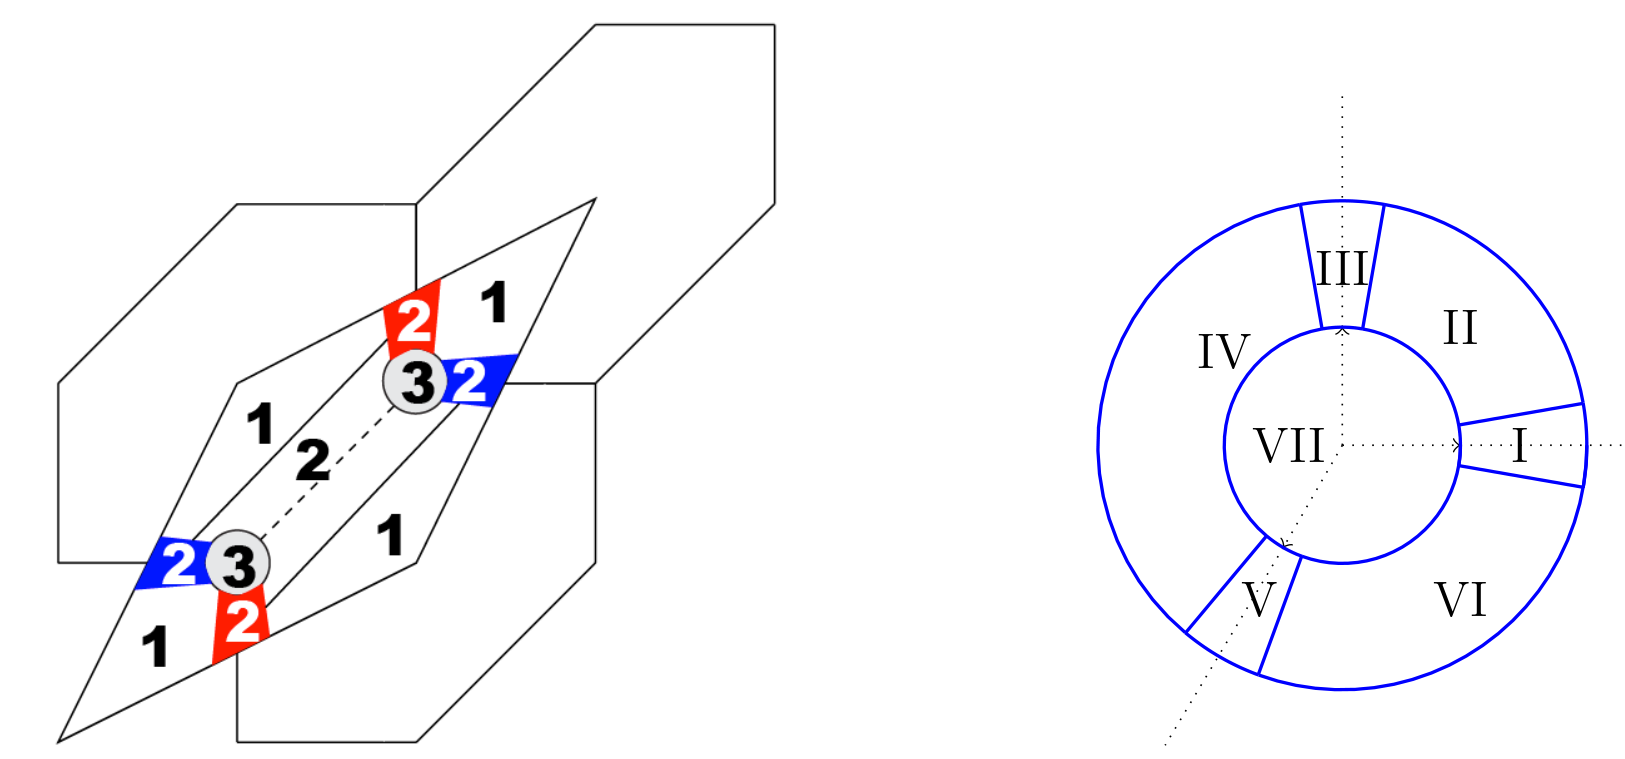
\includegraphics[width=0.86\textwidth]{figures/fig_2_1.png}
\caption{左（L）：所插值的势的数目。右（R）：顶点附近的放大区域。（原书 p.49）}
\label{fig:2-1}
\end{figure}

\medskip
\noindent\textbf{区域 I 的主项}\par
先看没有鼓包函数导数的项。它们应当给出正定矩阵，于是得到度量。随后只需证明：其余各项都能写成（鼓包函数的对数导数）乘（有界项）的形式，而后者只要把 $l$ 取够大就能任意小。首先回忆极坐标下的度量是
\[
\begin{pmatrix}
\partial^2_{r_x}F+\frac{1}{r_x}\partial_{r_x}F & \partial^2_{r_xr_y}F & \partial^2_{r_xr_z}F\\
\partial^2_{r_xr_y}F & \partial^2_{r_y}F+\frac{1}{r_y}\partial_{r_y}F & \partial^2_{r_yr_z}F\\
\partial^2_{r_xr_z}F & \partial^2_{r_yr_z}F & \partial^2_{r_z}F+\frac{1}{r_z}\partial_{r_z}F
\end{pmatrix}.
\]

% ===== 原书 p.50 =====
\begin{gather*}
F=f+\alpha_3d+\alpha_4\cdot\alpha_5\theta,\\
d\approx T^2\Big[r_x^2-\tfrac12(r_y^2+r_z^2)\Big],\\
\theta\approx T^2[r_y^2-r_z^2],\\
f\approx T^2[r_y^2+r_z^2].
\end{gather*}

注意 $r_x$ 处处以 $r_x^2$ 的形式出现，所以作用 $\partial^2_{r_xr_x}$ 等同于作用 $\partial_{r_x}/r_x$。下面列出不含 $\alpha_i$ 导数的项；为记号简便，下标 $x$ 表示 $\partial_{r_x}$：
\[
\begin{aligned}
&\begin{pmatrix}
2(f_{xx}+\alpha_3d_{xx}+\alpha_4\alpha_5\theta_{xx}) & f_{xy}+\alpha_3d_{xy}+\alpha_4\alpha_5\theta_{xy} & f_{xz}+\alpha_3d_{xz}+\alpha_4\alpha_5\theta_{xz}\\
\text{“} & 2(f_{yy}+\alpha_3d_{yy}+\alpha_4\alpha_5\theta_{yy}) & f_{yz}+\alpha_3d_{yz}+\alpha_4\alpha_5\theta_{yz}\\
\text{“} & \text{“} & 2(f_{zz}+\alpha_3d_{zz}+\alpha_4\alpha_5\theta_{zz})
\end{pmatrix}\\
&\qquad\approx T^2
\begin{pmatrix}
4\alpha_3 & 0 & 0\\
0 & 4-2\alpha_3+4\alpha_4\alpha_5 & 0\\
0 & 0 & 4-2\alpha_3-4\alpha_4\alpha_5
\end{pmatrix}.
\end{aligned}
\]

展开式中高阶项的导数会带 $Tr_*$ 变量，因而可以忽略。只要把区域稍微限制一下，这个矩阵就有下界：每个元素都有下界。鼓包函数到达边界时，确有一个坐标趋于零。不过在 $xy$ 平面里趋于零的是 $z$ 项，$xz$ 平面里同理是 $y$ 项。由于我们从底空间加上一项 $|xyz|^2$，离开零纤维处就有正定性。

\medskip
\noindent\textbf{区域 I 中含鼓包函数导数的项}\par
产生鼓包函数导数的项是 $\alpha_3(d_I)d_I$ 与 $\alpha_4(\theta_I)\alpha_5(d_I)\theta_I$。注意在 $r_x=r_y=r_z$ 附近的区域 I 中，$d$ 关于 $(Tr_x)^2$、$(Tr_y)^2$、$(Tr_z)^2$ 近似线性。

记号约定：本节令 $d\equiv d_I$。我们让求导所沿的变量在 $\{r_x,r_y,r_z\}$ 中变动，并把这组变量记作 $\{r_\star,r_\bullet\}\in\{r_x,r_y,r_z\}$。又，$'^{\log}$ 表示取对数导数 $d\alpha_3/d(\log(d_I))=\alpha_3'\cdot d$。下面的二阶导数计算对 $\alpha_5$ 同样适用；把 $d$ 换成 $\theta$ 后对 $\alpha_4$ 也适用。

% ===== 原书 p.51 =====
\begin{align*}
\frac{d^2\alpha_3}{d(\log d)}&=(\alpha_3'\cdot d)'\cdot d=(\alpha_3''\cdot d+\alpha_3')d\\
\Longrightarrow\quad\alpha_3''\cdot d+\alpha_3'&=\frac{1}{d}\cdot\frac{d^2\alpha_3}{d(\log d)^2}\\
\Longrightarrow\quad\alpha_3''&=\frac{1}{d^2}\left(\frac{d^2\alpha_3}{d(\log d)^2}-\frac{d\alpha_3}{d(\log d)}\right)
\end{align*}
% [Tutor Note: 第一行左端原文作 d^2α3 / d(log d)，按上下文应为 d^2α3 / d(log d)^2；照录不改。]

\transnote{本章的 ${\alpha_i'}^{\log}$ 一律指对数导数 $\alpha_i'\cdot d$（或 $\alpha_i'\cdot\theta$），量级为 $1/l$；而 ${\alpha_i''}^{\log}$ 指二阶对数导数，量级为 $1/l^2$。原书在这两个记号与普通导数之间来回换用，读式子时务必先看是哪种：后面的「小量乘有界量」估计全靠 $1/l$ 与 $1/l^2$ 的差别。}

\medskip
\noindent\textbf{$\alpha_3d$ 的导数}\par
一阶导数：$\frac{1}{r_\star}\partial_{r_\star}(\alpha_3d)$。其中 $\alpha_3'd={\alpha_3'}^{\log}$ 是对数导数，可以取得任意小。

二阶导数：$\alpha_3d$ 的二阶导数涉及 $r_\star\alpha_3'd$ 的一阶导数，其中含前面那样的 $\alpha_3'd$ 项，以及 $r_\star(\partial_\bullet d)(\alpha_3''d+\alpha_3')$ 乘以 $T$ 的幂，即正比于 $T^2r_\star r_\bullet(\alpha_3''d+\alpha_3')$，因为 $d$ 关于 $(Tr_x)^2,(Tr_y)^2,(Tr_z)^2$ 近似线性。于是得到
\[
\frac{T^2r_\star r_\bullet}{d}{\alpha_3''}^{\log}.
\]
把分子分母同除以 $r_x^2$，得
\[
\frac{(r_\star r_\bullet)/(r_x)^2}{1-\frac12\big((r_y/r_x)^2+(r_z/r_x)^2\big)},
\]
分母接近 $1$，分子小或等于 $1$，因为 $r_x\gg r_y,r_z$。于是得到有界量乘小量。因此只要 $l$ 固定且足够大，含 $\alpha_3$ 的导数都给出小项。下面写出计算。

\medskip
\noindent\textbf{$\alpha_3(d)\cdot d$ 的对角项：}\par
\begin{align*}
&d\approx T^2\Big[r_x^2-\frac12(r_y^2+r_z^2)\Big],\qquad
d_{r_\star}\approx\lambda T^2r_\star,\quad d_{r_\star r_\star}\approx\lambda T^2,\quad \lambda\in\{2,-1\},\\
&\Big(\frac{1}{r_\star}\partial_{r_\star}+\partial^2_{r_\star r_\star}\Big)(\alpha_3(d)\cdot d)
=\frac{1}{r_\star}\big(\alpha_3'd_{r_\star}d+\alpha_3(d)\cdot d_{r_\star}\big)\\
&\qquad+\big(\alpha_3''d_{r_\star}^2d+\alpha_3'd_{r_\star r_\star}d+2\alpha_3'(d)d_{r_\star}^2+\alpha_3(d)\cdot d_{r_\star r_\star}\big)\\
&\approx\frac{1}{r_\star}\big(\alpha_3'\lambda T^2r_\star d+\alpha_3(d)\cdot\lambda T^2r_\star\big)\\
&\qquad+\big(\alpha_3''(\lambda T^2r_\star)^2d+\alpha_3'\lambda T^2d+2\alpha_3'(d)(\lambda T^2r_\star)^2+\alpha_3(d)\cdot\lambda T^2\big)\\
&=\lambda T^2\big[\alpha_3'd+\alpha_3+\lambda T^2\alpha_3''r_\star^2\cdot d+\alpha_3'd+2\lambda T^2\alpha_3'r_\star^2+\alpha_3(d)\big]\\
&=2\lambda T^2\big[\alpha_3'\big(d+(\lambda-1)T^2r_\star^2\big)+T^2r_\star^2(\alpha_3''d+\alpha_3')\big]+2\lambda T^2\alpha_3\\
&=2\lambda T^2\Big[{\alpha_3'}^{\log}\Big(1+(\lambda-1)\frac{T^2r_\star^2}{d}\Big)+\frac{T^2r_\star^2}{d}{\alpha_3''}^{\log}\Big]+2\lambda T^2\alpha_3.
\end{align*}

% ===== 原书 p.52 =====
\[
{\alpha_3'}^{\log}\approx\frac{\Delta\alpha_3}{\Delta\log d}\approx\propto\frac{1}{l},
\qquad
{\alpha_3''}^{\log}\approx\propto\frac{1}{l^2}.
\]
\[
\frac{T^2r_\star^2}{d}\approx\frac{T^2r_\star^2}{T^2\big[r_x^2-\frac12(r_y^2+r_z^2)\big]}
=\frac{r_\star^2}{r_x^2-\frac12(r_y^2+r_z^2)}
=\frac{r_\star^2/r_x^2}{1-\frac12\Big(\frac{r_y^2}{r_x^2}+\frac{r_z^2}{r_x^2}\Big)}
\approx 1\ \text{或}\ 0\quad\because r_x\gg r_y,r_z.
\]

\medskip
\noindent\textbf{$\alpha_3(d)\cdot d$ 的非对角项，$\star\ne\bullet$：}\par
\begin{align*}
d_{r_\star r_\bullet}&=0\\
\partial^2_{r_\star r_\bullet}(\alpha_3\cdot d)&=\partial_{r_\star}\big(\alpha_3'd_{r_\bullet}d+\alpha_3(d)\cdot d_{r_\bullet}\big)\\
&=\alpha_3''d_{r_\star}d_{r_\bullet}d+\alpha_3'd_{r_\bullet r_\star}d+2\alpha_3'd_{r_\bullet}d_{r_\star}+\alpha_3\cdot d_{r_\bullet r_\star}\\
&=T^4\lambda\mu r_\star r_\bullet\alpha_3''d+0+2T^4\lambda\mu r_\star r_\bullet\alpha_3'+0,\qquad\lambda,\mu\in\{2,-1\}\\
&=T^4\lambda\mu\frac{r_\star r_\bullet}{d}\,d(\alpha_3''d+\alpha_3'+\alpha_3')\\
&=T^4\lambda\mu\frac{r_\star r_\bullet}{d}\big({\alpha_3''}^{\log}+{\alpha_3'}^{\log}\big)
\end{align*}
% [Tutor Note: 上面倒数第二行多出的因子 d 与末行不相容；照录不改。]
\[
\frac{T^2r_\star r_\bullet}{d}\approx\frac{r_\star r_\bullet/r_x^2}{1-\frac12\big((r_y/r_x)^2+(r_z/r_x)^2\big)}\approx 0\ \text{或}\ 1.
\]

又可以看到，鼓包函数的导数全是对数导数，所有项都被常数乘 $T^2/l$ 界住。

\medskip
\noindent\textbf{$\alpha_4\alpha_5\theta$ 的导数}\par
对 $\alpha_4\alpha_5\theta$，一阶导数项（除以求导所沿的变量后）含 $\alpha_5(\alpha_4'\theta)$，这是 $O(1)$ 项（回忆 $\alpha_5$ 从 $0$ 走到 $1$）乘一个对数导数；还含 $\alpha_4(\alpha_5'\theta)=\alpha_4\big({\alpha_5'}^{\log}\cdot\frac{\theta}{d}\big)$，因为 $\alpha_5$ 是 $d$ 的函数。所以要检查 $\theta/d$ 有界且与 $l$ 无关。除以 $r_x^2$ 后分子是小量、分母接近 $1$。因此这两项都没问题。

一阶导数给出 $r_\star\alpha_5(\alpha_4'\theta)$ 与 $r_\star\alpha_4(\alpha_5'\theta)$。把 $r_\star$ 对 $r_\bullet$ 求导，得到上一段已证为小的项；当 $\bullet\ne\star$ 时得零。于是把它提到前面，只对剩下的表达式求导。注意 $\alpha_4$ 是 $\theta$ 的函数，$\alpha_5$ 是 $d$ 的函数。
\begin{itemize}[leftmargin=2.2em,itemsep=0.25em]
\item $r_\star r_\bullet\alpha_4'\alpha_5'\theta=\dfrac{r_\star r_\bullet}{d}{\alpha_4'}^{\log}{\alpha_5'}^{\log}$。这里乘 $d$ 再除以 $d$，以便凑出 $\alpha_5$ 的对数导数。
\item $r_\star r_\bullet\alpha_5(\alpha_4''\theta+\alpha_4')=\alpha_5\cdot\dfrac{r_\star r_\bullet}{\theta}{\alpha_4''}^{\log}$。其中 $r_\bullet$ 来自 $\partial_\bullet\theta$。特别地，若 $r_\bullet=r_x$ 则得零，因为 $\theta\approx T^2[r_y^2-r_z^2]$，即 $\theta_{r_x}\approx0$。
\end{itemize}

% ===== 原书 p.53 =====
\begin{itemize}[leftmargin=2.2em,itemsep=0.25em]
\item $r_\star r_\bullet\alpha_4(\alpha_5''\theta)=\alpha_4\cdot\dfrac{r_\star r_\bullet}{d}\big({\alpha_5''}^{\log}-{\alpha_5'}^{\log}\big)\cdot\dfrac{\theta}{d}$。
\item $r_\star r_\bullet\alpha_4(\alpha_5')=\dfrac{r_\star r_\bullet}{d}\cdot\alpha_4{\alpha_5'}^{\log}$。
\end{itemize}

上面已看到 $T^2\frac{r_\star r_\bullet}{d}$、从而 $\frac{\theta}{d}$ 有界。于是只剩检验 $T^2\frac{r_\star r_\bullet}{\theta}$ 有界。另外，按上面的说明，分子含 $r_x$ 时得零；又由二阶偏导数对称，只需考虑分子不含 $r_x$ 的情形。因此要估计下列表达式：
\[
\frac{r_y^2}{r_y^2-r_z^2},\qquad
\frac{r_z^2}{r_y^2-r_z^2},\qquad
\frac{r_yr_z}{r_y^2-r_z^2}.
\]

我们看区域 I 的上半部分，那里 $r_y>r_z$。我们规定 $\alpha_4$ 在区域 $1<\left(\frac{r_y}{r_z}\right)^2<\frac1T$ 内取常值。于是 $\alpha_4$ 的支撑集是 $\left(\frac{r_y}{r_z}\right)^2>\frac1T$。特别地，
\[
\frac{1}{\left(\frac{r_y}{r_z}\right)^2-1}<\frac{1}{\frac1T-1}=\frac{T}{1-T}\approx T.
\]
所以这些项有界；把分子分母同除以 $r_z^2$ 即可看出。下面是具体计算。

对角项为 $\frac{1}{r_\bullet}\partial_{r_\bullet}+\partial^2_{r_\bullet r_\bullet}$，非对角项为 $\partial^2_{r_\bullet r_\star}$。
\begin{align*}
\theta&\approx T^2(r_y^2-r_z^2),\\
d&\approx T^2\big(r_x^2-\tfrac12(r_y^2+r_z^2)\big),\\
\theta_{r_\bullet}&\approx\lambda_\bullet T^2r_\bullet,\qquad\lambda_\bullet\in\{0,\pm2\},\\
d_{r_\bullet}&\approx\mu_\bullet T^2r_\bullet,\qquad\mu_\bullet\in\{2,-1\},\\
\frac{1}{r_\bullet}\partial_{r_\bullet}(\alpha_4\alpha_5\theta)
&=\frac{1}{r_\bullet}\big(\alpha_4'\theta_{r_\bullet}\alpha_5\theta+\alpha_4\alpha_5'd_{r_\bullet}\theta+\alpha_4\alpha_5\theta_{r_\bullet}\big)\\
&=T^2\Big(\lambda_\bullet{\alpha_4'}^{\log}\alpha_5+\mu_\bullet\alpha_4{\alpha_5'}^{\log}\frac{\theta}{d}+\lambda_\bullet\alpha_4\alpha_5\Big).
\end{align*}

% ===== 原书 p.54 =====
\begin{align*}
\partial^2_{r_\star r_\bullet}(\alpha_4\alpha_5\theta)
&=T^2\partial_{r_\star}\big[r_\bullet\lambda_\bullet\alpha_4'\theta\alpha_5+r_\bullet\mu_\bullet\alpha_4\alpha_5'\theta+r_\bullet\lambda_\bullet\alpha_4\alpha_5\big]\\
&=T^2\big[\partial_{r_\star}r_\bullet\lambda_\bullet\alpha_4'\theta\alpha_5
+T^2r_\bullet\lambda_\bullet\alpha_4''\theta_{r_\star}\theta\alpha_5\\
&\qquad+T^2r_\bullet\lambda_\bullet\alpha_4'\theta_{r_\star}\alpha_5
+T^2r_\bullet\lambda_\bullet\alpha_4'\theta\alpha_5'd_{r_\star}
+\partial_{r_\star}(r_\bullet)\alpha_4\alpha_5'\theta\\
&\qquad+T^2r_\bullet\mu_\bullet\alpha_4'\theta_{r_\star}\alpha_5'\theta
+T^2r_\bullet\mu_\bullet\alpha_4\alpha_5''d_{r_\star}\theta
+T^2r_\bullet\mu_\bullet\alpha_4\alpha_5'\theta_{r_\star}\\
&\qquad+\partial_{r_\star}(r_\bullet)\lambda_\bullet\alpha_4\alpha_5
+T^2r_\bullet\lambda_\bullet\alpha_4'\theta_{r_\star}\alpha_5
+T^2r_\bullet\lambda_\bullet\alpha_4\alpha_5'd_{r_\star}\big]\\
&=T^2\Big[\delta_{\bullet\star}\lambda_\bullet{\alpha_4'}^{\log}\alpha_5
+T^2\Big[\lambda_\bullet\lambda_\star\frac{r_\bullet r_\star}{\theta}\big({\alpha_4''}^{\log}-{\alpha_4'}^{\log}\big)\alpha_5\\
&\qquad+\lambda_\bullet\lambda_\star\frac{r_\bullet r_\star}{\theta}{\alpha_4'}^{\log}\alpha_5
+\lambda_\bullet\mu_\star\frac{r_\bullet r_\star}{d}{\alpha_4'}^{\log}{\alpha_5'}^{\log}\Big]\\
&\qquad+\delta_{\star\bullet}\frac{\theta}{d}\alpha_4{\alpha_5'}^{\log}
+\mu_\bullet\lambda_\star\frac{T^2r_\bullet r_\star}{d}{\alpha_4'}^{\log}{\alpha_5'}^{\log}\\
&\qquad+\frac{T^2r_\bullet r_\star\theta}{d^2}\alpha_4\big({\alpha_5''}^{\log}-{\alpha_5'}^{\log}\big)
+\mu_\bullet\lambda_\star\frac{T^2r_\bullet r_\star}{d}{\alpha_5'}^{\log}\\
&\qquad+\delta_{\star\bullet}\lambda_\bullet\alpha_4\alpha_5
+\lambda_\bullet\lambda_\star\frac{T^2r_\bullet r_\star}{\theta}{\alpha_4'}^{\log}\alpha_5
+\lambda_\bullet\mu_\star\frac{T^2r_\bullet r_\star}{d}\alpha_4{\alpha_5'}^{\log}\Big].
\end{align*}

我们看到 $T^2\frac{r_\bullet r_\star}{\theta}$、$T^2\frac{r_\bullet r_\star}{d}$、$\frac{\theta}{d}$ 如上都有界，且其中的导数都是对数导数。

\medskip
\noindent\textbf{把区域 III 与 V 调成与区域 I 一致}\par
区域 I 中 $r_x$ 是主导坐标。区域 III 中 $r_y$ 将主导，区域 V 中 $r_z$ 将主导。于是仿照 I，取 III 与 V 各半区域的相应数据。

\begin{figure}[htbp]
\centering
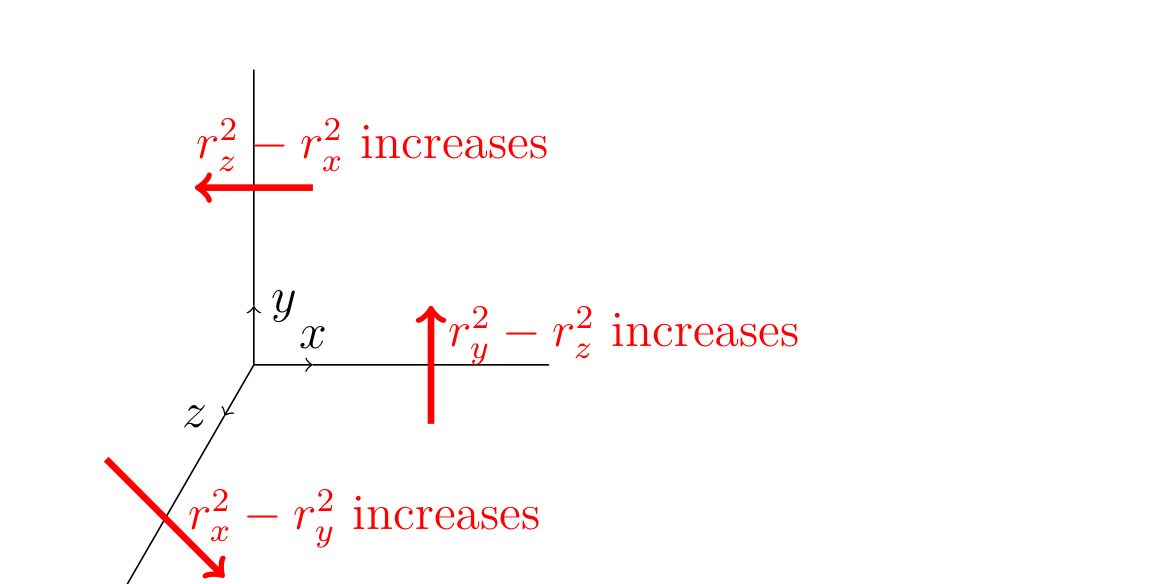
\includegraphics[width=0.62\textwidth]{figures/fig_2_2.png}
\caption{三个角方向。（原书 p.54）}
\label{fig:2-2}
\end{figure}

\begin{gather*}
g_{yz}=g_{yz}+\alpha_3(d_I)\cdot d_I+\alpha_4(\theta_I)\alpha_5(d_I)\cdot\theta_I\\
g_{yz}\approx T^2[r_y^2+r_z^2]\\
\theta_I\approx T^2[r_y^2-r_z^2]\\
d_I\approx T^2\Big[r_x^2-\frac12(r_y^2+r_z^2)\Big]
\end{gather*}
% [Tutor Note: 第一行左端原文写作 g_yz = g_yz + …，按上下文应为 F = g_yz + …；照录不改。]

% ===== 原书 p.55 =====
\begin{gather*}
g_{xy}=g_{xy}+\alpha_3(d_{III})\cdot d_{III}+\alpha_4(\theta_{III})\alpha_5(d_{III})\cdot\theta_{III}\\
g_{xy}\approx T^2[r_x^2+r_z^2]\\
\theta_{III}\approx T^2[r_z^2-r_x^2]\\
d_{III}\approx T^2\Big[r_y^2-\frac12(r_x^2+r_z^2)\Big]
\end{gather*}
\begin{gather*}
F_V=f_V+\alpha_3(d_V)\cdot d_V+\alpha_4(\theta_V)\alpha_5(d_V)\cdot\theta_V\\
f_V\approx T^2[r_x^2+r_y^2]\\
\theta_V\approx T^2[r_x^2-r_y^2]\\
d_V\approx T^2\Big[r_z^2-\frac12(r_x^2+r_y^2)\Big]
\end{gather*}

已知起点是 $\alpha_1g_{xy}+\alpha_2g_{xz}+(1-\alpha_1-\alpha_2)g_{yz}$，而终点应是 III 与 V 中的上述表达式；由于角方向与径向方向按上面的对称性确定，这就定下了 III 与 V 中 $\alpha_3$ 与 $\alpha_4\cdot\alpha_5$ 的取值。

区域 III 中要求
\begin{align*}
F&=g_{xy}+\alpha_3(d_{III})\cdot d_{III}+\alpha_4(\theta_{III})\alpha_5(d_{III})\cdot\theta_{III}\\
&=g_{xz}+\alpha_3\Big(\frac12(g_{yz}-g_{xz})+\frac12(g_{xy}-g_{xz})\Big)+\alpha_4\alpha_5(g_{yz}-g_{xy})\\
&=g_{xz}(1-\alpha_3)+g_{xy}\Big(\frac{\alpha_3}{2}-\alpha_4\alpha_5\Big)+g_{yz}\Big(\frac{\alpha_3}{2}+\alpha_4\alpha_5\Big)\\
&=\alpha_1g_{xy}+\alpha_2g_{xz}+(1-\alpha_1-\alpha_2)g_{yz}\\
&\Longrightarrow\quad\alpha_3=1-\alpha_2,\qquad\alpha_4\cdot\alpha_5=\frac12-\frac{\alpha_2}{2}-\alpha_1.
\end{align*}
% [Tutor Note: 上面第一行左端的 g_xy 与第二行的 g_xz 不一致；按 d_III 的展开，基项应为 g_xz。照录不改。]

区域 V 中要求
\begin{align*}
F&=f_V+\alpha_3(d_V)\cdot d_V+\alpha_4(\theta_V)\alpha_5(d_V)\cdot\theta_V\\
&=g_{xy}+\alpha_3\Big(\frac12(g_{xz}-g_{xy})+\frac12(g_{yz}-g_{xy})\Big)+\alpha_4\alpha_5(g_{xz}-g_{yz})\\
&=g_{xy}(1-\alpha_3)+g_{xz}\Big(\frac{\alpha_3}{2}+\alpha_4\alpha_5\Big)+g_{yz}\Big(\frac{\alpha_3}{2}-\alpha_4\alpha_5\Big)\\
&=\alpha_1g_{xy}+\alpha_2g_{xz}+(1-\alpha_1-\alpha_2)g_{yz}\\
&\Longrightarrow\quad\alpha_3=1-\alpha_1,\qquad\alpha_4\cdot\alpha_5=\alpha_2-\frac12+\frac{\alpha_1}{2}.
\end{align*}

% ===== 原书 p.56 =====
两种情形中 $\alpha_3$ 都从 $2/3$ 走到 $1$，$\alpha_4$ 都从 $-1/2$ 走到 $1/2$，$\alpha_5$ 则从 $0$ 到 $1$ 给它作缩放。既然一切都在 $(r_x,r_y,r_z)$ 下对称，前面的计算对 $f+\alpha_3d+\alpha_4\alpha_5\theta$ 照旧成立。现在的问题在于：$\alpha_{\ge3}$ 是 $d$ 与 $\theta$ 的函数，而这两个变量在三个区域中各有不同定义。因此我们要把 $d$ 坐标沿区域 II、IV、VI 拼接起来。

之所以只需拼接 $d$，是因为在奇数区域边界处 $\alpha_4$ 已经变平到 $1/2$ 或 $-1/2$，而 $\alpha_3,\alpha_5$ 只依赖 $d$。于是再取一个从 $0$ 到 $1$ 的鼓包函数 $\alpha_6$，在偶数区域里加入越来越多的 $\theta$ 坐标，从而在 $d$ 的两种定义之间插值。归纳一下：在 II、IV、VI 中，$\alpha_3$ 与 $\alpha_5$ 是 $d$ 的函数，而 $d$ 又是 $\alpha_6(\theta_{\text{even}})\cdot\theta_{\text{even}}$ 的函数。于是对 $r_x,r_y,r_z$ 求导时，链式法则要用两层。

\medskip
\noindent\textbf{区域 IIA 的主项}\par
先取不含鼓包函数导数的项。它们构成区域 II 上度量的非退化部分；其余各项我们会证明可以取得足够小。因为一切非鼓包的量都关于 $(Tr_x)^2$、$(Tr_y)^2$、$(Tr_z)^2$ 近似线性，所以仍有 $\frac{1}{r_x}\partial_{r_x}=\partial^2_{r_xr_x}$。回忆 $2/3\le\alpha_3\le1$，$0\le\alpha_5,\alpha_6\le1$。先修正第一行中的 $\phi$ 项。
\transnote{原文此处夹有作者的工作批注「Fix $\phi$ terms in first line.」，语义不明；照录为「先修正第一行中的 $\phi$ 项」。}

\begin{align*}
F&\approx T^2\Big[\big(r_y^2+r_z^2-\alpha_6(\theta_{II})\cdot r_y^2\big)
+\alpha_3(d_{IIA})\cdot\Big(r_x^2-\frac12(r_y^2+r_z^2)+\frac32\alpha_6(\theta_{II})\cdot r_y^2\Big)\\
&\qquad+\frac12\alpha_5(d_{IIA})\cdot\big(r_y^2-r_z^2-\alpha_6(\theta_{II})\cdot r_y^2\big)\Big]
\end{align*}

非对角项 $\partial^2_{r_\bullet r_\star}$（$\star\ne\bullet$）为零，因为对非鼓包函数求导就是对某个 $r_*^2$ 求导。对角项有 $\frac{1}{r_*}\partial_{r_*}+\partial^2_{r_*r_*}=2\partial^2_{r_*r_*}$，作用在 $(Tr_*)^2$ 上得 $2T^2$。于是矩阵的 $(*,*)$ 元中，主项是 $4T^2$ 乘 $r_*^2$ 的系数。$y$ 那一项还要核对。
\begin{align*}
x:\quad &T^2(4\alpha_3)\ge T^2\frac83,\\
y:\quad &T^2(4-4\alpha_6-2\alpha_3+6\alpha_3\alpha_6+2\alpha_5-2\alpha_5\alpha_6)
=T^2\big[4+(2-2\alpha_6)(\alpha_5-\alpha_3)+4\alpha_6(\alpha_3-1)\big]\\
&\ge T^2\big[4+2(0-2/3)+4(-1/3)\big]=T^2\cdot\frac43,\\
z:\quad &T^2(4-2\alpha_3-2\alpha_5).
\end{align*}

注意当 $\alpha_3=\alpha_5=1$ 时 $z$ 项趋于零。不过在 $\alpha_3,\alpha_5$ 与 $1$ 保持距离的区域里它有下界。在它趋于 $1$ 的区域，我们从底空间给 $F$ 加上一项 $|xyz|^2$，以维持非退化性。由于在加这一项的区域里 $xyz$ 有正的下界，求偏导数后得到的仍是正定的。

% ===== 原书 p.57 =====
\medskip
\noindent\textbf{区域 IIA 中含鼓包函数导数的项}\par
下面证明含鼓包函数导数的项可以取得很小。备查：
\begin{gather*}
F\approx\big(g_{yz}-\alpha_6\cdot(Tr_y)^2\big)+\alpha_3(d_{IIA})d_{IIA}
+\frac12\alpha_5(d_{IIA})\cdot\big((Tr_y)^2-(Tr_z)^2-\alpha_6(Tr_y)^2\big)\\
g_{yz}\approx T^2[r_y^2+r_z^2]\\
d_I\approx T^2\Big[r_x^2-\frac12(r_y^2+r_z^2)\Big]\\
d_{IIA}\approx T^2\Big[r_x^2-\frac12(r_y^2+r_z^2)\Big]+\frac32\alpha_6(\log r_y-\log r_x)\cdot(Tr_y)^2\\
\theta_I\approx T^2[r_y^2-r_z^2]\\
\theta_{II}=\log(r_y/r_x)
\end{gather*}

$F$ 中的鼓包函数项是：$\alpha_6\cdot(Tr_y)^2$、$\alpha_3\cdot d_{IIA}$、$\{\alpha_5(Tr_*)^2\}_{*=y,z}$、$\alpha_5\alpha_6\cdot(Tr_y)^2$。

第 1 项：$\alpha_6(\log(r_y/r_x))\cdot(Tr_y)^2$。

\medskip
\noindent 一阶导数（除以 $r_\star$）：
\begin{align*}
\frac{1}{r_x}\partial_{r_x}\big[\alpha_6(\log r_y-\log r_x)(Tr_y)^2\big]
&=-\frac{1}{r_x^2}\alpha_6'\cdot(Tr_y)^2=-T^2\cdot\frac{r_y^2}{r_x^2}\alpha_6',
\qquad\Big|\frac{r_y^2}{r_x^2}\Big|<1\\
\frac{1}{r_y}\partial_{r_y}\big[\alpha_6(\log r_y-\log r_x)(Tr_y)^2\big]
&=\frac{1}{r_y^2}\alpha_6'\cdot(Tr_y)^2+\alpha_6\cdot(2T^2r_y)=T^2\alpha_6'+2T^2\alpha_6r_y\\
\frac{1}{r_z}\partial_{r_z}\big[\alpha_6(\log r_y-\log r_x)(Tr_y)^2\big]&=0\\
\alpha_6'&\approx\propto\frac1l
\end{align*}

于是这一项的一阶导数给出的鼓包函数导数项都能取得很小。

\medskip
\noindent 二阶导数 $\partial^2_\bullet$：
\begin{align*}
\partial^2_{r_xr_x}(\alpha_6(Tr_y)^2)&=\partial_{r_x}\Big(-\frac{(Tr_y)^2}{r_x}\alpha_6'\Big)
=\frac{(Tr_y)^2}{r_x^2}(\alpha_6'+\alpha_6'')\\
&<T^2(\alpha_6'+\alpha_6'')\approx\propto T^2\Big(\frac1l+\frac1{l^2}\Big),\ \text{小}\\
\partial^2_{r_xr_y}(\alpha_6(Tr_y)^2)&=\partial_{r_y}\Big(-\frac{(Tr_y)^2}{r_x}\alpha_6'\Big)
=\frac{-T^2r_y}{r_x}(2\alpha_6'+\alpha_6''),\\
&\qquad\text{范数}<T^2(2\alpha_6'+\alpha_6'')\\
\partial^2_{r_yr_y}(\alpha_6(Tr_y)^2)&=\partial_{r_y}\big(T^2\alpha_6'r_y+2T^2\alpha_6r_y^2\big)\\
&=T^2(\alpha_6'+\alpha_6''+2\alpha_6'r_y+4\alpha_6r_y)<T^2(3\alpha_6'+\alpha_6''+4\alpha_6r_y)
\end{align*}

因为区域 II 中 $r_y$ 很小。注意一阶导数 $\alpha_6'$ 从 $0$ 增到 $l/2$ 中点处的最大值 $1/l+\epsilon$，因此斜率的变化约为 $1/l^2$，仍然很小。（确切地说是 $(1/l+\epsilon)(2/l)$。）所以 $\alpha_6r_y^2$ 这一项没有问题。

第 2 项：$\alpha_3(d_{IIA})d_{IIA}$。

% ===== 原书 p.58 =====
\medskip
\noindent\textbf{一阶导数。}$\frac{1}{r_\star}\partial_{r_\star}(\alpha_3d_{IIA})=(\alpha_3'd_{IIA}+\alpha_3)\cdot\frac{d_{IIA,\star}}{r_\star}$。下面是 $d_{IIA}$ 的偏导数。
\begin{align*}
d_{IIA}&\approx T^2\Big[r_x^2-\frac12(r_y^2+r_z^2)\Big]+\frac32\alpha_6(\log r_y-\log r_x)\cdot(Tr_y)^2\\
\frac{(d_{IIA})_x}{r_x}&=\frac{T^2}{r_x}\Big[2r_x+\frac32\Big(\alpha_6'\cdot\frac{-1}{r_x}\cdot r_y^2\Big)\Big]
=T^2\Big[2+\frac32\Big(\alpha_6'\cdot\frac{-r_y^2}{r_x^2}\Big)\Big]\\
\frac{(d_{IIA})_y}{r_y}&=\frac{T^2}{r_y}\Big[-r_y+\frac32\Big(\alpha_6'\cdot\frac1{r_y}\cdot r_y^2+2r_y\alpha_6\Big)\Big]
=T^2\Big[-1+\frac32(\alpha_6'+2\alpha_6)\Big]\\
\frac{(d_{IIA})_z}{r_z}&=\frac{T^2}{r_z}[-r_z]=-T^2
\end{align*}

于是 $\frac{1}{r_\star}\partial_{r_\star}(\alpha_3d_{IIA})=(\alpha_3'd_{IIA}+\alpha_3)\cdot\frac{d_{IIA,\star}}{r_\star}$ 中的项如下：
\begin{itemize}[leftmargin=2.2em,itemsep=0.2em]
\item 用 $\frac{d_{IIA,\star}}{r_\star}$ 中可能出现的项乘 $\alpha_3'd_{IIA}$：
 \begin{itemize}[leftmargin=1.8em,itemsep=0.15em]
 \item $\alpha_3'd_{IIA}$：$\star$ 任意，来自各个 $\frac{d_{IIA,\star}}{r_\star}$ 的常数项；
 \item $\alpha_3'd_{IIA}\alpha_6$：$\star=y$，因为 $\alpha_6$ 只出现在 $\star=y$ 的导数里；
 \item $\alpha_3'd_{IIA}\alpha_6'$：$\star=y$，同上；
 \item $\alpha_3'd_{IIA}\alpha_6'\cdot\left(\frac{r_y}{r_x}\right)^2$：仅 $\star=x$。
 \end{itemize}
\item 用 $\frac{d_{IIA,\star}}{r_\star}$ 乘 $\alpha_3$：
 \begin{itemize}[leftmargin=1.8em,itemsep=0.15em]
 \item $\alpha_3$：$\star$ 任意；
 \item $\alpha_3\alpha_6$：$\star=y$；
 \item $\alpha_3\alpha_6'$：$\star=y$；
 \item $\alpha_3\alpha_6'\cdot\left(\frac{r_y}{r_x}\right)^2$：$\star=x$。
 \end{itemize}
\end{itemize}

这里每一项都没问题：要么得到 ${\alpha_3'}^{\log}=\alpha_3'd_{IIA}$，要么得到 $\alpha_6$ 的通常导数；后者可能乘上 $(r_y/r_x)^2$，而区域 IIA 中 $r_x>r_y$，所以导数项可以取得很小。

\medskip
\noindent\textbf{二阶导数项。} 对上列每个一阶导数项求导。设 $P$ 是上表中的一项。因为前面除以了 $r_\star$，现在要对 $r_\star P$ 求导。用微分算子 $D=\partial_{r_\bullet}$ 与乘积法则得 $D(r_\star)P+r_\star D(P)$。第一项给出 $0$ 或 $1$ 乘 $P$，而上表已说明每个 $P$ 都小。所以只需对上表 8 种 $P$ 考察 $r_\star D(P)$。

\transnote{这里把二阶导数的检验压缩成「只需看 $r_\star D(P)$」，理由是 $D(r_\star)$ 只给出 $0$ 或 $1$，而 $1$ 倍的那部分已知是小量。抓这一点是本段长清单的目的：$P$ 一共 8 种，若逐一从头算二阶导数会失控，先剥掉 $D(r_\star)P$ 才把工作量化到 8 个小计算。}

% ===== 原书 p.59 =====
\medskip
\noindent\textbf{1.}\ $P=\alpha_3'd_{IIA}$。

这一项通过 $r_\star\partial_{r_\bullet}(P)$ 给 $\partial^2_{r_\star r_\bullet}(F)$ 作贡献，即
\[
r_\star\partial_{r_\bullet}(\alpha_3'd_{IIA})
=r_\star\alpha_3''\cdot(d_{IIA})_\bullet\cdot d_{IIA}+r_\star\alpha_3'(d_{IIA})_\bullet
=\frac{r_\star(d_{IIA})_\bullet}{d_{IIA}}{\alpha_3''}^{\log},
\]
\[
(d_{IIA})_\bullet\ \text{的取值}:\ \Big\{T^2r_\bullet,\ T^2\alpha_6r_y,\ T^2\alpha_6'r_y,\ T^2\alpha_6'\frac{r_y^2}{r_x}\Big\}<T^2r_\bullet,
\quad\because\alpha_6\le1,\ \alpha_6'\approx\propto\frac1l,\ \frac{r_y}{r_x}<1,
\]
\[
\begin{aligned}
\frac{T^2r_\star r_\bullet}{d_{IIA}}
&\approx\frac{r_\star r_\bullet}{r_x^2-\frac12(r_y^2+r_z^2)+\frac32\alpha_6r_y^2}
=\frac{r_\star r_\bullet/r_x^2}{1-\frac12\big((r_y/r_x)^2+(r_z/r_x)^2\big)+\frac32\alpha_6(r_y/r_x)^2}\\
&\approx\frac{r_\star r_\bullet}{r_x^2}\in\{0,1\}
\quad\because r_x\gg r_y,r_z\ \text{在区域 IIA}.
\end{aligned}
\]
\[
\therefore\quad r_\star\partial_{r_\bullet}(P)=\frac{r_\star(d_{IIA})_\bullet}{d_{IIA}}{\alpha_3''}^{\log}\approx(\text{有界})\cdot\frac1{l^2}.
\]

\medskip
\noindent\textbf{2.}\ $P=\alpha_3'd_{IIA}\alpha_6$，来自对 $F$ 先按 $y$ 求导，即 $\partial_{r_y}(F)$。
\begin{align*}
r_y\partial_{r_\bullet}(\alpha_3'd_{IIA}\alpha_6)
&=r_y\partial_{r_\bullet}(\alpha_3'd_{IIA})\cdot\alpha_6+r_y(\alpha_3'd_{IIA})\cdot\partial_{r_\bullet}(\alpha_6)\\
&=(\text{上一情形})\cdot\alpha_6\pm{\alpha_3'}^{\log}\alpha_6'\cdot cr_y,\qquad c\in\Big\{\frac1{r_x},\frac1{r_y},0\Big\}\\
&=\text{小}+\text{小}.
\end{align*}

\medskip
\noindent\textbf{3.}\ $\alpha_3'd_{IIA}\alpha_6'$，来自先按 $y$ 求导。与第 2 条相同，把 $\alpha_6$ 换成 $\alpha_6'$。

\medskip
\noindent\textbf{4.}\ $\alpha_3'd_{IIA}\alpha_6'\cdot\left(\frac{r_y}{r_x}\right)^2$，来自先按 $x$ 求导。
\begin{align*}
r_x\partial_{r_\bullet}\Big(\alpha_3'd_{IIA}\alpha_6'\cdot\Big(\frac{r_y}{r_x}\Big)^2\Big)
&=r_x\partial_{r_\bullet}(\alpha_3'd_{IIA}\alpha_6')\cdot\Big(\frac{r_y}{r_x}\Big)^2
+r_x(\alpha_3'd_{IIA}\alpha_6')\cdot\partial_{r_\bullet}\Big(\Big(\frac{r_y}{r_x}\Big)^2\Big)\\
&=\frac{r_y}{r_x}\cdot r_y\partial_{r_\bullet}(\alpha_3'd_{IIA}\alpha_6')
\pm({\alpha_3'}^{\log}\alpha_6')\cdot cr_x,\qquad c\in\Big\{\frac{2r_y^2}{r_x^3},\frac{2r_y}{r_x^2},0\Big\}\\
&=(\text{小})(\text{上一情形})+(\text{小})\Big(\frac{r_y}{r_x}\Big)^i,\qquad i\in\{1,2\}\\
&=\text{小}\quad\because r_x\gg r_y.
\end{align*}

\medskip
\noindent\textbf{5.}\ $P=\alpha_3$：它出现在 $F$ 对任一变量的一阶导数中。

再求一次导得 $r_\star\partial_{r_\bullet}\alpha_3=r_\star\alpha_3'(d_{IIA})_\bullet={\alpha_3'}^{\log}\cdot(r_\star(d_{IIA})_\bullet)/d_{IIA}$。所以要 $(r_\star(d_{IIA})_\bullet)/d_{IIA}$ 有界；第 1 条已检验过。

\medskip
\noindent\textbf{6.}\ $P=\alpha_3\alpha_6$：它出现在 $F$ 对 $y$ 的一阶导数中。
\[
r_y\partial_{r_\bullet}(\alpha_3\alpha_6)=r_y\big((\alpha_3)_\bullet\alpha_6+\alpha_3(\alpha_6)_\bullet\big).
\]

% ===== 原书 p.60 =====
含 $\alpha_3$ 导数的那项已归入上一情形。第二项给出 $\alpha_3\alpha_6'$ 乘 $\{0,\ r_y/r_x\approx0,\ 1\}$ 之一，于是这一项是有界量乘小量，同样小。

\medskip
\noindent\textbf{7.}\ $P=\alpha_3\alpha_6'$：$\star=y$。把上一情形中的 $\alpha_6$ 换成 $\alpha_6'$。

\medskip
\noindent\textbf{8.}\ $P=\alpha_3\alpha_6'(r_y/r_x)^2$：$\star=x$。计算与第 4 条完全相同，只是「已检验」的部分现在是 $\alpha_3\alpha_6'$ 而不是 $\alpha_3'd_{IIA}\alpha_6'$。

至此完成了 $\alpha_3(d_{IIA})d_{IIA}$ 一阶与二阶导数的检验。

\[
\text{第 3 项：}\ \alpha_5\cdot(Tr_*)^2,\qquad *\in\{y,z\}
\]

我们照搬上面 $\alpha_3\cdot d_{IIA}$ 的论证，只把第二项里的 $d_{IIA}$ 换成 $(Tr_*)^2$。

\medskip
\noindent\textbf{一阶导数。}$\frac{1}{r_\star}\partial_{r_\star}(\alpha_5(Tr_*)^2)=\frac{1}{r_\star}\alpha_5'(d_{IIA})_\star(Tr_*)^2+\alpha_5\cdot\frac{((Tr_*)^2)_\star}{r_\star}$。而 $(Tr_*)^2$ 的偏导数是 $\frac{1}{r_\star}\partial_{r_\star}((Tr_*)^2)=2T^2$ 或 $0$。

于是 $\frac{1}{r_\star}\partial_{r_\star}(\alpha_5(Tr_*)^2)$ 中的非零项是 $2T^2\alpha_5$ 与
\[
\frac{1}{r_\star}\alpha_5'(d_{IIA})_\star(Tr_*)^2={\alpha_5'}^{\log}\frac{T^2r_*^2(d_{IIA})_\star}{d_{IIA}r_\star}.
\]
注意 $\frac{T^2r_*^2}{d_{IIA}}$ 与 $\frac{(d_{IIA})_\star}{r_\star}$ 都有界；后者已在第 2、3 条中检验。前者：
\[
\frac{r_*^2}{r_x^2-\frac12(r_y^2+r_z^2)+\frac32\alpha_6r_y^2}
=\frac{r_*^2/r_x^2}{1-\frac12\big((r_y/r_x)^2+(r_z/r_x)^2\big)+\frac32\alpha_6(r_y/r_x)^2}
\approx0\quad\because r_x\gg r_y,r_z.
\]
注意 $*\in\{y,z\}$。所以一阶导数没问题：要么是非鼓包函数的导数，要么是有界量乘小对数导数。

\medskip
\noindent\textbf{二阶导数项。} 逐个对一阶导数项求导。它们是 $\alpha_5'(d_{IIA})_*(Tr_*)^2$ 与 $2T^2r_*\alpha_5$。设 $Pr_*$ 是其中一项，即上一条中考虑的 $P$。用微分算子 $D=\partial_{r_\bullet}$ 与乘积法则得 $D(r_*)P+r_*D(P)$。第一项给出 $0$ 或 $1$ 乘 $P$，上面已说明每个 $P$ 都小。所以只需对这 2 种 $P$ 考察 $r_*D(P)$。

\medskip
\noindent\textbf{1.}\ $P=\alpha_5'(Tr_*)^2\frac{(d_{IIA})_*}{r_*}$。这涉及下面的项：把 $\alpha_5'(Tr_*)^2$ 乘上 $\frac{(d_{IIA})_*}{r_*}$ 中出现的四类项，再逐类检验由此产生的二阶导数。

% ===== 原书 p.61 =====
\medskip
\noindent（i）$\alpha_5'(Tr_*)^2$：这一项通过 $r_\star\partial_{r_\bullet}(P)$ 给 $\partial^2_{r_\star r_\bullet}(F)$ 作贡献，即
\begin{align*}
r_\star\partial_{r_\bullet}(\alpha_5'(Tr_*)^2)
&=r_\star\alpha_5''\cdot(d_{IIA})_\bullet\cdot(Tr_*)^2+r_\star\alpha_5'((Tr_*)^2)_\bullet\\
&=\big({\alpha_5''}^{\log}-{\alpha_5'}^{\log}\big)\frac{r_\star(d_{IIA})_\bullet(Tr_*)^2}{d_{IIA}^2}
+{\alpha_5'}^{\log}\frac{2T^2r_\bullet r_\star}{d_{IIA}}.
\end{align*}
已检验有界：$\frac{r_\star(d_{IIA})_\bullet}{d_{IIA}}$（第 1 条）、$\frac{(Tr_*)^2}{d_{IIA}}$（上面）、$\frac{T^2r_\bullet r_\star}{d_{IIA}}$（第 1 条）。因此
\[
\therefore\quad r_\star\partial_{r_\bullet}(\alpha_5'(Tr_*)^2)=(\text{小})(\text{有界})+(\text{小})(\text{有界}).
\]

\medskip
\noindent（ii）$\alpha_5'(Tr_*)^2\alpha_6$：来自对 $F$ 先按 $y$ 求导，即 $\partial_{r_y}(F)$。
\begin{align*}
r_y\partial_{r_\bullet}(\alpha_5'(Tr_*)^2\alpha_6)
&=r_y\partial_{r_\bullet}(\alpha_5'(Tr_*)^2)\cdot\alpha_6+r_y(\alpha_5'(Tr_*)^2)\cdot\partial_{r_\bullet}(\alpha_6)\\
&=(\text{上一情形})\cdot\alpha_6\pm{\alpha_5'}^{\log}\frac{(Tr_*)^2}{d_{IIA}}\alpha_6'\cdot cr_y,
\qquad c\in\Big\{\frac1{r_x},\frac1{r_y},0\Big\}\\
&=(\text{小})(\text{有界})+(\text{小})(\text{有界}).
\end{align*}

\medskip
\noindent（iii）$\alpha_5'(Tr_*)^2\alpha_6'$：来自先按 $y$ 求导。与上一情形相同，把 $\alpha_6$ 换成 $\alpha_6'$。

\medskip
\noindent（iv）$\alpha_5'(Tr_*)^2\alpha_6'\cdot\left(\frac{r_y}{r_x}\right)^2$：来自先按 $x$ 求导。
\begin{align*}
r_x&\partial_{r_\bullet}\Big(\alpha_5'(Tr_*)^2\alpha_6'\Big(\frac{r_y}{r_x}\Big)^2\Big)\\
&=r_x\partial_{r_\bullet}(\alpha_5'(Tr_*)^2\alpha_6')\cdot\Big(\frac{r_y}{r_x}\Big)^2
+r_x(\alpha_5'(Tr_*)^2\alpha_6')\cdot\partial_{r_\bullet}\Big(\Big(\frac{r_y}{r_x}\Big)^2\Big)\\
&=\frac{r_y}{r_x}\cdot r_y\partial_{r_\bullet}(\alpha_5'(Tr_*)^2\alpha_6')\\
&\qquad\pm\Big({\alpha_5'}^{\log}\frac{(Tr_*)^2}{d_{IIA}}\alpha_6'\Big)\cdot cr_x,
\qquad c\in\Big\{\frac{2r_y^2}{r_x^3},\frac{2r_y}{r_x^2},0\Big\}\\
&=(\text{小})(\text{上一情形})+(\text{小})\Big(\frac{r_y}{r_x}\Big)^i,\qquad i\in\{1,2\}\\
&=\text{小}\quad\because r_x\gg r_y.
\end{align*}

\medskip
\noindent\textbf{2.}\ $P=2T^2\alpha_5$：它出现在 $F$ 对任一变量的一阶导数中。

再求一次导得 $r_\star\partial_{r_\bullet}2T^2\alpha_5=r_\star2T^2\alpha_5'(d_{IIA})_\bullet=2T^2{\alpha_5'}^{\log}\cdot(r_\star(d_{IIA})_\bullet)/d_{IIA}$。所以要 $(r_\star(d_{IIA})_\bullet)/d_{IIA}$ 有界；第 1 条已检验过。

至此完成了 $\alpha_5(d_{IIA})d_{IIA}$ 一阶与二阶导数的检验。$F$ 中还有一类项，需要检验它的一阶与二阶导数。

\[
\text{第 4 项：}\ \alpha_5\alpha_6\cdot(Tr_y)^2
\]
\begin{align*}
&\frac{1}{r_\star}\partial_{r_\star}(\alpha_5(Tr_y)^2)\cdot\alpha_6+\alpha_5(Tr_y)^2\cdot\frac{1}{r_\star}\partial_{r_\star}\alpha_6\\
&\qquad=(\text{前面})\cdot\alpha_6\pm\alpha_5(Tr_y)^2\cdot\frac{c}{r_\star^2}\alpha_6'.
\end{align*}
就第二项而言：$\star=z\Longrightarrow c=0$；$\star=x\Longrightarrow\approx0$，因 $r_x\gg r_y$；$\star=y\Longrightarrow\frac{r_y^2}{r_\star^2}=1$。

% ===== 原书 p.62 =====
一阶导数至此没问题。最后检验二阶导数。
\begin{align*}
&\partial_{r_\bullet}\big[\partial_{r_\star}(\alpha_5(Tr_y)^2)\cdot\alpha_6+\alpha_5(Tr_y)^2\cdot\partial_{r_\star}(\alpha_6)\big]\\
&\qquad=\partial^2_{r_\bullet r_\star}(\alpha_5(Tr_y)^2)\cdot\alpha_6+\partial_{r_\star}(\alpha_5(Tr_y)^2)\partial_{r_\bullet}\alpha_6
+\partial_{r_\bullet}(\alpha_5(Tr_y)^2)\partial_{r_\star}\alpha_6+\alpha_5(Tr_y)^2\cdot\partial_{r_\bullet}\partial_{r_\star}(\alpha_6).
\end{align*}
第 1 项由前面关于 $\alpha_5(Tr_y)^2$ 的检验可知没问题。

第 2、3 项：
\begin{align*}
\partial_{r_\star}(\alpha_5(Tr_y)^2)\cdot\partial_{r_\bullet}\alpha_6
&=\Big({\alpha_5'}^{\log}\frac{(d_{IIA})_\star}{d_{IIA}}(Tr_y)^2+2\alpha_5T^2\delta_{y\star}r_y\Big)\cdot\frac{\pm1}{r_x\ \text{或}\ r_y}\cdot\alpha_6'\\
&=\pm\Big[T^2{\alpha_5'}^{\log}\frac{(d_{IIA})_\star r_y}{d_{IIA}}\cdot\frac{r_y}{r_x\ \text{或}\ r_y}\cdot\alpha_6'
+2\alpha_5T^2\frac{r_y}{r_x\ \text{或}\ r_y}\cdot\alpha_6'\Big].
\end{align*}

第 4 项：
\begin{align*}
\alpha_5(Tr_y)^2\partial_{r_\bullet}\Big(\frac{\alpha_6'}{r_x\ \text{或}\ r_y}\Big)
&=\alpha_5(Tr_y)^2\Big[\alpha_6''\cdot\frac{\pm1}{r_x\ \text{或}\ r_y}\cdot\frac{1}{r_x\ \text{或}\ r_y}
-\alpha_6'\frac{1}{r_x^2\ \text{或}\ r_y^2}\Big]\\
&=T^2\alpha_5\alpha_6''\frac{\pm r_y^2}{r_x^2,\ r_xr_y,\ \text{或}\ r_y^2}
-T^2\alpha_5\alpha_6'\frac{r_y^2}{r_x^2\ \text{或}\ r_y^2}\\
&=\text{小},\qquad\because r_x\gg r_y.
\end{align*}
\[
\Longrightarrow\quad\partial_{r_\bullet}\partial_{r_\star}\big(\alpha_5\alpha_6\cdot(Tr_y)^2\big)=(\text{小})\quad\text{由第 1 条}.
\]

归结起来：含鼓包函数导数的项都可以取得任意小，因为它们乘上的表达式有界（或是 $\alpha_3$、$\alpha_5$ 的对数导数，或是 $\alpha_6$ 的通常导数）。于是得到正定的形式：不含鼓包函数导数的项是 $O(1)$，因而占主导，而前面已证明它们给出正定的东西。

\medskip
\noindent\textbf{确定区域 IIB 上的函数}\par
我们刚在区域 IIA 中检验过，由对称性在区域 IIC 中也成立；同理 IVA、C 与 VIA、C 也成立。把 $r_x\leftrightarrow r_y$ 互换即得 IIC，此时下标 I 变成 III。

区域 IIA：
\begin{gather*}
F\approx\big(g_{yz}-\alpha_6\cdot(Tr_y)^2\big)+\alpha_3(d_{IIA})d_{IIA}
+\frac12\alpha_5(d_{IIA})\cdot\big((Tr_y)^2-(Tr_z)^2-\alpha_6(Tr_y)^2\big)\\
g_{yz}\approx T^2[r_y^2+r_z^2]\\
d_I\approx T^2\Big[r_x^2-\frac12(r_y^2+r_z^2)\Big]\\
d_{IIA}\approx T^2\Big[r_x^2-\frac12(r_y^2+r_z^2)\Big]+\frac32\alpha_6(\log r_y-\log r_x)\cdot(Tr_y)^2\\
\theta_I\approx T^2[r_y^2-r_z^2]\\
\theta_{II}=\log(r_y/r_x)
\end{gather*}

% ===== 原书 p.63 =====
区域 IIC：
\begin{gather*}
F=\big(g_{xy}-\alpha_6\cdot(Tr_y)^2\big)+\alpha_3(d_{IIC})d_{IIC}
+\frac12\alpha_5(d_{IIC})\cdot\big((Tr_x)^2-(Tr_z)^2-\alpha_6(Tr_x)^2\big)\\
g_{xy}\approx T^2[r_x^2+r_z^2]\\
d_{III}\approx T^2\Big[r_y^2-\frac12(r_x^2+r_z^2)\Big]\\
d_{IIC}\approx T^2\Big[r_y^2-\frac12(r_x^2+r_z^2)\Big]+\frac32\alpha_6(\log r_x-\log r_y)\cdot(Tr_x)^2\\
\theta_{III}\approx T^2[r_x^2-r_z^2]\\
\theta_{II}=\log(r_y/r_x)
\end{gather*}

在区域 IIA 的末端、$\alpha_6\equiv1$ 时，得到：
\begin{gather*}
F\approx\big(g_{yz}-(Tr_y)^2\big)+\alpha_3(d_{IIA})d_{IIA}+\frac12\alpha_5(d_{IIA})\cdot\big(-(Tr_z)^2\big)\\
g_{yz}\approx T^2[r_y^2+r_z^2]\\
d_I\approx T^2\Big[r_x^2-\frac12(r_y^2+r_z^2)\Big]\\
d_{IIA}\approx T^2\Big[r_x^2+r_y^2-\frac12r_z^2\Big]
\end{gather*}

在区域 IIC 的末端、$\alpha_6\equiv1$ 时（$\alpha_6$ 仍看作 $\theta_{II}$ 的函数）：
\begin{gather*}
F\approx\big(g_{xy}-(Tr_y)^2\big)+\alpha_3(d_{IIC})d_{IIC}+\frac12\alpha_5(d_{IIC})\cdot\big(-(Tr_z)^2\big)\\
g_{xy}\approx T^2[r_x^2+r_z^2]\\
d_{III}\approx T^2\Big[r_y^2-\frac12(r_x^2+r_z^2)\Big]\\
d_{IIC}\approx T^2\Big[r_y^2+r_x^2-\frac12r_z^2\Big]
\end{gather*}

所以 $F$ 在区域 IIB 上应当等于它在 IIA 与 IIC 两端所取的值。注意两端上 $d_{IIA}$ 与 $d_{IIC}$ 相等，于是取 $d_{IIB}$ 为这个共同的近似：
\[
d_{IIB}:=T^2\Big[r_x^2+r_y^2-\frac12r_z^2\Big].
\]
两端的非鼓包函数都是 $(Tr_z)^2$。最后，乘 $\alpha_5$ 的因子关于 $x$、$y$ 也对称，即 $-(Tr_z)^2$。

\transnote{\transnote{这里能只插值 $d$ 而不管其他变量，靠的是两条同时成立：一、偶数区域里 $\alpha_3,\alpha_5$ 只依赖 $d$；二、奇数区域边界上 $\alpha_4$ 已变平为常数 $\pm1/2$，故它带来的差别只通过 $d$ 进门。漏掉任一条，$F$ 在 IIB 上就不止一个待插值的自由度。}}

区域 IIB：
\begin{gather*}
F\approx T^2r_z^2+\alpha_3(d_{IIB})d_{IIB}+\frac12\alpha_5(d_{IIB})\cdot(-r_z^2)\\
d_{IIB}\approx T^2\Big[r_x^2+r_y^2-\frac12r_z^2\Big]
\end{gather*}

% ===== 原书 p.64 =====
注意在另一端，IIA 应当接到区域 I，IIC 应当接到区域 III。在区域 IIA 的末端、$\alpha_6\equiv0$ 时，得到：
\begin{gather*}
F\approx g_{yz}+\alpha_3(d_{IIA})d_{IIA}+\frac12\alpha_5(d_{IIA})\cdot\theta_I\\
g_{yz}\approx T^2[r_y^2+r_z^2]\\
\theta_I\approx(Tr_y)^2-(Tr_z)^2\\
d_I\approx T^2\Big[r_x^2-\frac12(r_y^2+r_z^2)\Big]\\
d_{IIA}\approx T^2\Big[r_x^2-\frac12(r_y^2+r_z^2)\Big]\\
\therefore\quad d_I=d_{IIA}
\end{gather*}

在区域 IIC 的末端、$\alpha_6\equiv0$ 时：
\begin{gather*}
F\approx g_{xy}+\alpha_3(d_{IIC})d_{IIC}+\frac12\alpha_5(d_{IIC})\cdot(-\theta_{III})\\
g_{xy}\approx T^2[r_x^2+r_z^2]\\
\theta_{III}\approx(Tr_z)^2-(Tr_x)^2\\
d_{III}\approx T^2\Big[r_y^2-\frac12(r_x^2+r_z^2)\Big]\\
d_{IIC}\approx T^2\Big[r_y^2-\frac12(r_x^2+r_z^2)\Big]\\
\therefore\quad d_{III}=d_{IIC}
\end{gather*}

注意此处的区域 III 角，与区域 III 另一半上得到的角互为相反数。这是因为两种角都要等于区域 II 中部的 $-(Tr_z)^2$ 才能拼接。若在坐标 $(x'',y'',z'')$ 下按与 $(x,y,z)$ 相同的方式定义辛形式，则形式能正确拼接。只剩区域 IIB 需要检验，它的行为与前面检验过的区域不同。

\medskip
\noindent\textbf{区域 IIB}\par
区域 IIB 具有而 IIA、C 没有的特征有两条：1）$r_x$ 与 $r_y$ 从 $r_x\gg r_y$ 变到 $r_y\gg r_x$，途中经过 $r_x=r_y$；2）$\alpha_6\equiv1$。$r_x,r_y,r_z$ 仍然都很小，所以凯勒势的近似仍然可用：
\begin{gather*}
F\approx T^2r_z^2+\alpha_3(d_{IIB})d_{IIB}+\frac12\alpha_5(d_{IIB})\cdot\big(-(Tr_z)^2\big)\\
d_{IIB}\approx T^2\Big[r_x^2+r_y^2-\frac12r_z^2\Big]
\end{gather*}

把上面的计算对区域 IIB 重做一遍，即对 $\alpha_3(d_{IIA})\cdot d_{IIA}$ 与 $\alpha_5\cdot(Tr_z)^2$，看看哪些地方用到了 $r_x\gg r_y$。在区域 IIB 中我们知道的是 $r_x,r_y\gg r_z$。

% ===== 原书 p.65 =====
\[
\text{第 1 项：}\ \alpha_3(d_{IIB})d_{IIB}
\]
\noindent\textbf{一阶导数。}\ $\frac{1}{r_\star}\partial_{r_\star}(\alpha_3d_{IIB})=(\alpha_3'd_{IIB}+\alpha_3)\cdot\frac{d_{IIB,\star}}{r_\star}$。下面给出 $d_{IIB}$ 的偏导数。
\begin{gather*}
d_{IIB}\approx T^2\Big[r_x^2+r_y^2-\frac12r_z^2\Big]\\
\frac{(d_{IIB})_x}{r_x}\approx\frac{T^2}{r_x}(2r_x)=\frac{T^2}{2}\\
\frac{(d_{IIB})_y}{r_y}\approx\frac{T^2}{2}\\
\frac{(d_{IIB})_z}{r_z}\approx-\frac{T^2}{4}
\end{gather*}
% [Tutor Note: 按 d_{IIB}=T^2[rx^2+ry^2-rz^2/2] 直接求导应为 2T^2、2T^2、-T^2；原文第一行中间式 (T^2/r_x)(2r_x) 也等于 2T^2，却写成 T^2/2，三处一致地差 4 倍，疑原文漏写因子 1/4，或不一致；照录不改，只作提示。]
于是 $\frac{1}{r_\star}\partial_{r_\star}(\alpha_3d_{IIB})=(\alpha_3'd_{IIB}+\alpha_3)\cdot\frac{d_{IIB,\star}}{r_\star}$ 中的项正比于 $\alpha_3'd_{IIB}$（对数导数，因而是小量）与 $\alpha_3$（不带导数）。所以一阶导数没问题。

\noindent\textbf{二阶导数项。}\ 对每个一阶导数项再求导。设 $P$ 是上表中的一个项。我们要求 $r_\star P$ 的导数，因为上面已除以 $r_\star$。于是用乘积法则，取微分算子 $D=\partial_{r_\bullet}$，得 $D(r_\star)P+r_\star D(P)$。第一项给出 $0$ 或 $1$ 倍的 $P$，而每个 $P$ 都已由上面那条说明知道是小量。所以只需考虑上列 $P$ 的 2 种取法下的 $r_\star D(P)$。

\medskip
\noindent 1.\ $P=\alpha_3'd_{IIB}$

这一项通过 $r_\star\partial_{r_\bullet}(P)$ 给 $\partial^2_{r_\star r_\bullet}(F)$ 作贡献，即
\begin{align*}
r_\star\partial_{r_\bullet}(\alpha_3'd_{IIB})
&=r_\star\alpha_3''\cdot(d_{IIB})_\bullet\cdot d_{IIB}+r_\star\alpha_3'(d_{IIB})_\bullet
=\frac{r_\star(d_{IIB})_\bullet}{d_{IIB}}{\alpha_3''}^{\log},\\
(d_{IIB})_\bullet\ \text{型项}&:\ T^2r_\bullet,\\
\frac{T^2r_\star r_\bullet}{d_{IIB}}
&\approx\frac{r_\star r_\bullet}{r_x^2+r_y^2-\frac12r_z^2}
=\frac{r_\star r_\bullet/r_x^2}{1+(r_y/r_x)^2-\frac12(r_z/r_x)^2}
\approx\frac{r_\star r_\bullet/r_x^2}{1+(r_y/r_x)^2},\\
(\star,\bullet)\in\{&(r_x,r_x),(r_x,r_z),(r_z,r_z)\}\ \Longrightarrow\ \frac{r_\star r_\bullet}{r_x^2}\in\{1,\ \text{小}\}\quad\because r_x\gg r_z,\\
(\star,\bullet)&=(r_y,r_z)\ \Longrightarrow\ \frac{r_yr_z}{r_x^2}<\frac{r_y}{r_x},\\
(\star,\bullet)\in\{&(r_x,r_y),(r_y,r_y)\}\ \text{时只须估计：}\ \frac{a}{1+a^2},\ \frac{a^2}{1+a^2},\quad a=r_y/r_x,\\
&\frac{a^2}{1+a^2}\le1,\quad a<1\Longrightarrow\frac{a}{1+a^2}<1,\quad a\ge1\Longrightarrow\frac{a}{1+a^2}\le\frac{a^2}{1+a^2}\le1,\\
&\therefore\quad r_\star\partial_{r_\bullet}(\alpha_3'd_{IIB})=(\text{有界})\cdot(\text{小}).
\end{align*}

% ===== 原书 p.66 =====
\medskip
\noindent 2.\ $P=\alpha_3$

再求一次导得 $r_\star\partial_{r_\bullet}\alpha_3=r_\star\alpha_3'(d_{IIB})_\bullet={\alpha_3'}^{\log}\cdot(r_\star(d_{IIB})_\bullet)/d_{IIB}$。所以要 $(r_\star(d_{IIB})_\bullet)/d_{IIB}$ 有界；上一段刚检验过。

\[
\text{第 2 项：}\ \alpha_5\cdot(Tr_z)^2
\]
我们照上面 $\alpha_3\cdot d_{IIB}$ 的论证走一遍，只把第二项中的 $d_{IIB}$ 换成 $(Tr_z)^2$。

\noindent\textbf{一阶导数。}\ $\frac{1}{r_\star}\partial_{r_\star}(\alpha_5(Tr_z)^2)=\frac{1}{r_\star}\alpha_5'(d_{IIB})_\star(Tr_z)^2+\alpha_5\cdot\frac{((Tr_z)^2)_\star}{r_\star}$。其中 $(Tr_z)^2$ 的偏导数为 $\frac{1}{r_\star}\partial_{r_\star}((Tr_z)^2)=2T^2$ 或 $0$。

于是 $\frac{1}{r_\star}\partial_{r_\star}(\alpha_5(Tr_z)^2)$ 中的非零项为 $2T^2\alpha_5$ 与
\[
\frac{1}{r_\star}\alpha_5'(d_{IIB})_\star(Tr_z)^2={\alpha_5'}^{\log}\frac{T^2r_z^2(d_{IIB})_\star}{d_{IIB}\cdot r_\star}.
\]
注意 $\frac{T^2r_z^2}{d_{IIB}}$ 与 $\frac{(d_{IIB})_\star}{r_\star}$ 都有界。后者近似为常数，因为 $d_{IIB}$ 对 $r_x^2$、$r_y^2$、$r_z^2$ 近似线性。前者：
\[
\frac{r_z^2}{r_x^2+r_y^2-\frac12r_z^2}
=\frac{r_z^2/r_x^2}{1+r_y^2/r_x^2-\frac12(r_z/r_x)^2}
\approx\frac{r_z^2/r_x^2}{1+r_y^2/r_x^2}\approx0\quad\because r_x\gg r_z.
\]
所以一阶导数没问题。

\noindent\textbf{二阶导数项。}\ 对每个一阶导数项再求导。这些项是 $\alpha_5'(d_{IIB})_\star(Tr_z)^2$ 与 $2T^2r_\star\alpha_5$。设 $Pr_\star$ 是其中之一，即上一段中考虑过的 $P$。于是用乘积法则，取微分算子 $D=\partial_{r_\bullet}$，得 $D(r_\star)P+r_\star D(P)$。第一项给出 $0$ 或 $1$ 倍的 $P$，而每个 $P$ 已由上面那条说明知道是小量。所以只需考虑这 2 种 $P$ 下的 $r_\star D(P)$。

% ===== 原书 p.67 =====
\medskip
\noindent 1.\ $P=\alpha_5'(Tr_z)^2\frac{(d_{IIB})_\star}{r_\star}$。只须考虑 $\alpha_5'(Tr_z)^2$，因为 $\frac{(d_{IIB})_\star}{r_\star}$ 是常数。
\begin{align*}
r_\star\partial_{r_\bullet}(\alpha_5'(Tr_z)^2)
&=r_\star\alpha_5''\cdot(d_{IIB})_\bullet\cdot(Tr_z)^2+r_\star\alpha_5'((Tr_z)^2)_\bullet\\
&=\big({\alpha_5''}^{\log}-{\alpha_5'}^{\log}\big)\frac{r_\star(d_{IIB})_\bullet(Tr_z)^2}{d_{IIB}^2}
+{\alpha_5'}^{\log}\frac{2T^2r_zr_\star}{d_{IIB}}.
\end{align*}
已检验有界：$\frac{r_\star(d_{IIB})_\bullet}{d_{IIB}}$、$\frac{(Tr_z)^2}{d_{IIB}}$（见上文）。
\begin{align*}
\frac{T^2r_zr_\star}{d_{IIB}}
&\approx\frac{r_zr_\star/r_x^2}{1+(r_y/r_x)^2-\frac12(r_z/r_x)^2}
\approx\frac{r_zr_\star/r_x^2}{1+(r_y/r_x)^2}<\frac{r_\star/r_x}{1+(r_y/r_x)^2},\\
&\star=x\ \Longrightarrow\ \text{有界};\qquad
\star=y\ \Longrightarrow\ a/(1+a^2)\ \text{如上界};\qquad
\star=z\ \Longrightarrow\ \text{小},\\
&\therefore\quad r_\star\partial_{r_\bullet}(\alpha_5'(Tr_z)^2)=(\text{小})(\text{有界})+(\text{小})(\text{有界}).
\end{align*}

\medskip
\noindent 2.\ $P=2T^2\alpha_5$：它出现在 $F$ 对任一变量的一阶导数中。

再求一次导得 $r_\star\partial_{r_\bullet}2T^2\alpha_5=r_\star2T^2\alpha_5'(d_{IIB})_\bullet=2T^2{\alpha_5'}^{\log}\cdot(r_\star(d_{IIB})_\bullet)/d_{IIB}$。所以要 $(r_\star(d_{IIB})_\bullet)/d_{IIB}$ 有界；上面已检验过。

正定性的计算到此完成。下面把细节补全：检验对数导数有足够空间，办法是给出 $r_x,r_y,r_z$ 的近似值，从而给出 $\theta$ 与 $d$ 各变量的近似值，确保它们的 $\log_T$ 值变化量与 $l$ 成正比。

\transnote{「对数导数有足够空间」是本章全部估计的支点：鼓包函数的导数只能靠「小量乘有界量」压住，而小量来自对数导数，所以必须确认每个鼓包函数在其支撑集内自变量确实走了 $l$ 量级的 $\log_T$ 跨度；否则 $\alpha_i'$ 会退化成 $O(1)$，估计失效。}

\medskip
\noindent\textbf{$\C^3$ 卡的剩余部分}\par
在区域 I 与区域 IIA 之间的区域，起作用的鼓包函数只有 $\alpha_3$ 与 $\alpha_5$，它们可变化的余地与上面检验过的相同，且仍有 $r_x\gg r_y,r_z$，所以前面所有估计都适用。

\subsection{证明 $\omega$ 非退化：$\C^3$ 卡之外}

% ===== 原书 p.68 =====
以上计算都用到近似，因为 $r_x,r_y,r_z$ 在 $\C^3$ 卡附近都很小。无界多面体的每个顶点附近都有带很小坐标的坐标系，所以在每个顶点附近局部定义辛形式。（可以类比的例子是 $\PP^1$ 上 $0$ 附近的坐标 $z$ 与 $\infty$ 附近的坐标 $w=1/z$。$z$ 在 $w$ 卡里确实很大，但 $z$ 与 $w$ 小得一样，因此可以取 $\log(1+|\text{coord}|^2)$，它在两个卡里看起来相同。）于是剩下的检验是：辛形式沿例如 $z$ 轴正定地拼接。

沿 $z$ 轴的绿色区域里已没有 $d_V$ 坐标，因为决定它的鼓包函数 $\alpha_3$、$\alpha_5$ 的支撑集已结束。但仍有一个角坐标，允许我们在不带撇的坐标下于 $g_{xz}$ 与 $g_{yz}$ 之间插值，或在左下顶点的三重撇坐标下于 $g_{x'''z'''}$ 与 $g_{y'''z'''}$ 之间插值。所以要检验的是：只有 $\alpha_4$ 起作用、$r_z$ 很大时，形式仍正定。注意没有鼓包函数时正定性成立：我们或者在区域 VII 中，那里是标准凯勒势；或者在三点爆破的 $\PP^2$ 的环簇的 $\PP^2(3)$ 中心，那里有可从格点读出的自然势。

\begin{figure}[htbp]
\centering
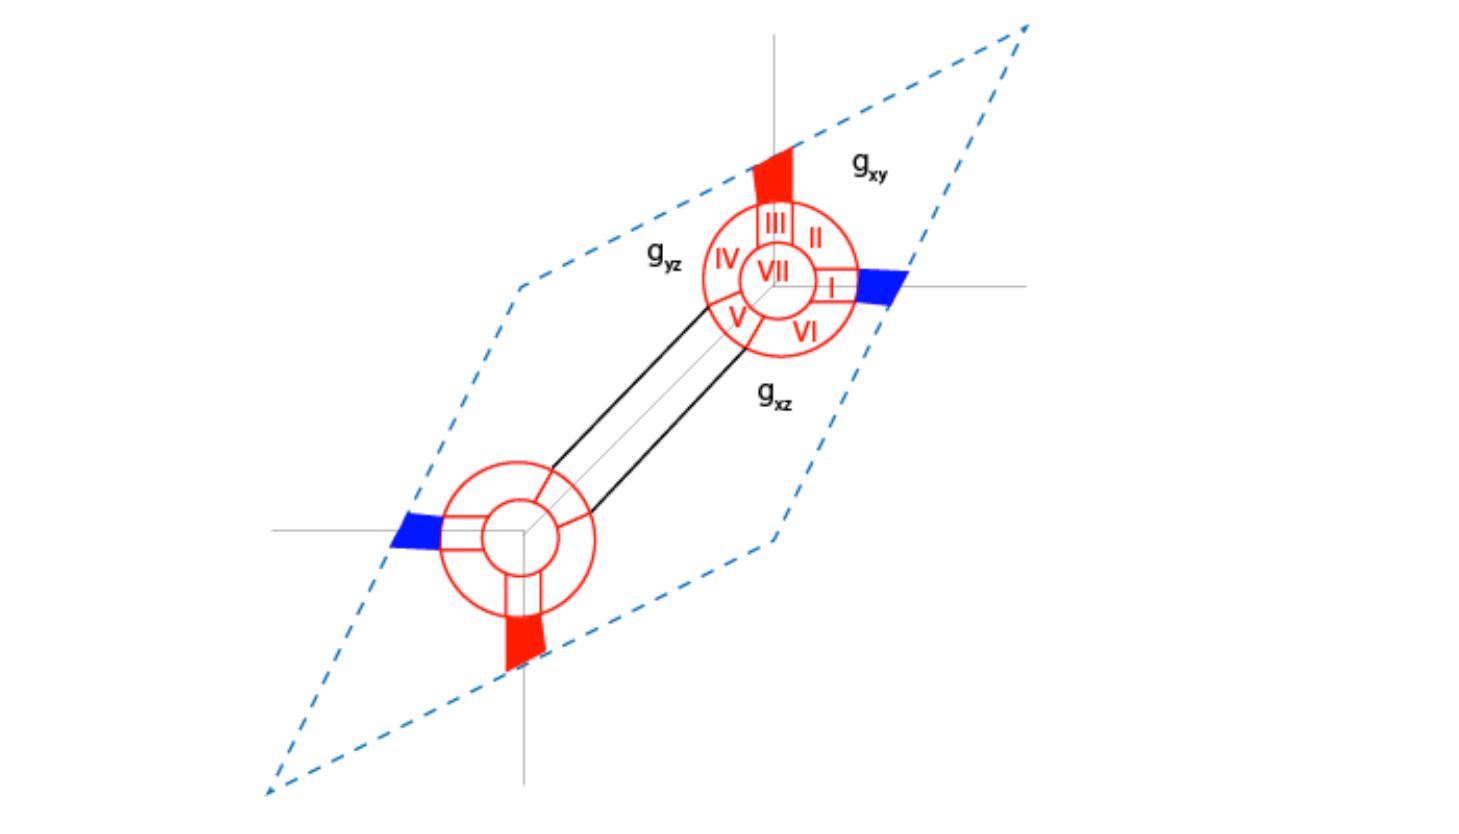
\includegraphics[width=0.62\textwidth]{figures/fig_2_3.png}
\end{figure}

\transnote{此图在原书中没有图号与图注，故这里也不加 \texttt{\textbackslash caption}，以免与原文只有图 2.1、图 2.2 的编号体系冲突。图中虚线框是无界多面体，两个红色小圆是顶点附近的小坐标卡，红色与蓝色箭头分别标出该处起作用的 $g$ 分量。}

还须检验 $|z|$ 很大时得到正定的东西。注意坐标上的等价关系 $\sim$ 正是把坐标看成环簇卡时得到的过渡映射。以 $\PP^2$ 为例：$\C\times\C^*$ 作为各卡的重叠部分落在所有卡内；它在一个卡中的嵌入是 $(u,v)$，在另一个卡中是 $(v^{-1},uv^{-1})$，这就告诉我们过渡映射把 $(u,v)$ 送到另一个。在我们的情形里，先不处理齐次坐标，图景直接给出环簇坐标上的过渡映射。

% ===== 原书 p.69 =====
具体地说，我们希望当 $|v_0|\neq0$ 时找出 $z$ 坐标的中点。固定一个纤维时，这对应于 $(\C^*)^2$ 到自身的环簇卡拼接。那个 $z$ 坐标映到 $T^{-2}z^{-1}$，起点为 $T^{l/3}$。所以我们仍然是把两份 $\C^*$ 互相粘起来，只不过其中一份从半径为 $T^{l/3}$ 的圆开始，而不是只挖掉原点。中点仍是 $T^{-1}$，只是我们粘的是比 $\PP^1$ 情形多挖了一些的平面。于是 $|z|$ 从 $T^{l/3}$ 变到 $T^{-1}$。由于上一项刚检验过的拼接性质，只须检验一半。

\transnote{「只须检验一半」用的正是 $z\mapsto T^{-2}z^{-1}$ 的拼接线对称性：两半的估计互为镜像，若一半上形式正定，另一半随之成立；漏掉这一句会把计算量算成两倍。}

据此检验鼓包函数导数有界。凯勒势形如 $(f+d)+\alpha_4(\theta)\cdot\theta$，所以只须检验 $\alpha_4(\theta)\cdot\theta$ 的导数。这一项可以用上面的计算，理由如下：虽然 $|z|\le T^{-1}$，但可设 $|x|$ 与 $|y|$ 很小。于是 $|T^2xz|\le|Tx|$、$|T^2yz|\le|Ty|$，这些量都很小，它们的对数又有小尺度近似：
\begin{align*}
\theta&=\phi_x-\phi_y\\
&=\log_T(1+|Tx|^2)-\log_T(1+|T^2yz|^2)-\log_T(1+|Ty|^2)+\log_T(1+|T^2xz|^2)\\
&\approx2|Tx|^2-2|Ty|^2\\
\frac{1}{r_*}\frac{\partial}{\partial r_*}(\alpha_4\theta)&=(\alpha_4'\theta+\alpha_4)\frac{\theta_*}{r_*}\\
\frac{\partial}{\partial r_\bullet}(\alpha_4'\theta\theta_*)
&=\alpha_4''\theta_\bullet\theta\theta_*+\alpha_4'\theta_\bullet\theta_*+\alpha_4'\theta\theta_{*\bullet}\\
&=\big(\alpha_4''\theta^2+\alpha_4'\theta\big)\cdot\frac{\theta_\bullet\theta_*}{\theta}
+{\alpha_4'}^{\log}\theta_{*\bullet}\\
\frac{\partial}{\partial r_\bullet}(\alpha_4\theta_*)
&=\alpha_4'\theta_\bullet\theta_*+\alpha_4\theta_{*\bullet}\\
&={\alpha_4'}^{\log}\frac{\theta_\bullet\theta_*}{\theta}+\alpha_4\theta_{*\bullet}
\end{align*}
于是需要估计下面三项，然后检查对数导数有足够空间：
\begin{itemize}[leftmargin=2.2em,itemsep=0.25em]
\item $\frac{\theta_*}{r_*}$：
\[
\frac{\theta_x}{r_x}\approx4T^2,\qquad \frac{\theta_y}{r_y}\approx-4T^2,\qquad \frac{\theta_z}{r_z}\approx0.
\]
\item $\frac{\theta_\bullet\theta_*}{\theta}$ 意味着要考虑 $\frac{r_\bullet r_*}{r_x^2-r_y^2}$，因此需要尺寸约束，使 $\alpha_4$ 的支撑集避开 $r_x=r_y$ 的区域。回想上面已挖掉窄条 $T<(r_x/r_y)^2<1/T$。又因 $\theta$ 近似为 $2T^2(r_x^2-r_y^2)$，只要 $*$ 与 $\bullet$ 都不是 $z$，这一项就近似为零。与前面一样，按两个变量中较大者分别除以 $r_x^2$ 或 $r_y^2$，于是分子至多为 $1$，分母由约束 $T<(r_x/r_y)^2<1/T$ 有正下界。
\item 除 $*=\bullet$ 外，$\theta_{*\bullet}$ 近似为零；而 $*=\bullet$ 时它是常数，故有界。
\end{itemize}
注意对数导数会有足够空间，因为 $r_x$、$r_y$ 很小时 $\theta\approx2T^2(r_x^2-r_y^2)$；这一点在早先按 $\theta\approx T^2(r_x^2-r_y^2)$ 检验时已经做过。
